%% Bernoulli [BJ] submission -- single-file build.
%% GENERATED by manuscript/bernoulli/build_bj.py from manuscript/sections-v2/.
%% Edit the sources in manuscript/sections-v2/, then re-run the script.
\documentclass[bj,authoryear]{imsart}

%% imsart loads natbib itself; do not load it again.
%% authoryear matches the Bernoulli template default and supports the
%% \citet{...} calls used in the prose (imsart-number.bst does not).
\usepackage{amsmath,amssymb,amsthm,mathtools,bm,booktabs,graphicx}
\usepackage{microtype}
\usepackage[section]{placeins}
\graphicspath{{../}}

\startlocaldefs
\theoremstyle{plain}
\newtheorem{theorem}{Theorem}[section]
\newtheorem{proposition}[theorem]{Proposition}
\newtheorem{corollary}[theorem]{Corollary}
\newtheorem{lemma}[theorem]{Lemma}
\DeclareMathOperator*{\esssup}{ess\,sup}
\DeclareMathOperator*{\argmax}{arg\,max}
\newcommand{\A}{A}\newcommand{\I}{I_\varepsilon}
\newcommand{\M}{\mathcal{M}}\newcommand{\Pp}{\mathbb P}
\newcommand{\E}{\mathbb E}\newcommand{\R}{\mathbb R}
\newcommand{\gmax}{\gamma^\star}
\endlocaldefs

\begin{document}

\begin{frontmatter}
\title{Tail-Index Sure Independence Screening for
High-Dimensional Heavy-Tailed Regression}
\runtitle{Tail-Index Sure Independence Screening}

%% Affiliations: Podgorny per alexpodgorny.fr (postdoc, ENSAI Rennes and
%% IRMAR UMR 6625, equipe de statistique); Pommeret per his public profile
%% (LISN, Universite Paris-Saclay/CNRS). Confirm before submission.
\begin{aug}
\author[A]{\inits{A.}\fnms{Alex}~\snm{Podgorny}\ead[label=e1]{alex.podgorny@univ-rennes2.fr}}
\author[B]{\inits{L.}\fnms{Luc}~\snm{Pommeret}\ead[label=e2]{luc.pommeret@universite-paris-saclay.fr}}
\address[A]{ENSAI and IRMAR (UMR CNRS 6625), Universit\'e de Rennes\printead[presep={,\ }]{e1}}
\address[B]{LISN, Universit\'e Paris-Saclay, CNRS\printead[presep={,\ }]{e2}}
\end{aug}

\begin{abstract}
We propose a marginal screen for the covariates that determine a positive
conditional tail index, designed for problems where the dimension $p$ is large
relative to the number of observations informative about the tail. The screen
rests on one geometric fact: after projection onto a single coordinate, the
conditional distribution is a mixture whose tail is governed by its heaviest
component, so the projected tail index is the upper envelope of the tail-index
surface along the corresponding fibre. Inactive coordinates produce flat
envelopes at the global maximum $\gmax$, while an active coordinate whose
fibres miss the global argmax set depresses the envelope; ranking coordinates
by the average projected index therefore separates active variables from
noise, and we characterize exactly which active coordinates a marginal screen
can see, rather than assuming a generic signal-strength condition. We estimate
the envelope with empirical-rank local Hill profiles. Ranks give every
coordinate the same deterministic window geometry, which removes the covariate
density conditions that fixed-dimension projected-tail theory requires and
permits exact finite-sample union bounds over a diverging number of
coordinates: the maximal score error over $p$ coordinates is
$O_{\Pp}(\sqrt{\log(pn)/(n\alpha h)})$, where $\alpha$ is the local tail
fraction, $h$ the rank bandwidth, and $n\alpha h$ the effective local extreme
sample size. Sure screening and exact recovery follow when
$\log(pn)=o(n\alpha h\Delta_{\min}^2)$, so a polynomially growing dimension is
affordable whenever the local extreme count dominates the logarithm of the
dimension. The algorithm costs $O(pn\log n)$ time and $O(n)$ working memory,
under a second per screen at $(n,p)=(2000,1000)$. A rank-aggregated version,
taking the minimum rank over a block of nine neighbouring tunings, stabilizes
the ranking against the choice of the smoothing parameters. Simulations across
$p\in\{500,1000,2000\}$, including a model whose scale is driven by a
correlated cluster of twenty inactive covariates, show when screening on
the tail index differs from screening on a fixed high quantile: the
cluster fills the leading positions of moderate-level quantile screens,
whose contamination clears at extreme levels only at a severe variance
cost, while the leading positions of the aggregated tail screen remain
on the active set. An application to violent-crime rates in 1{,}993
U.S. communities, with $p=99$ continuous predictors against an
effective tail sample of about $200$, illustrates the method in the
regime it is designed for, and separates predictors of the limiting
exponent from predictors of a high quantile on real data. The uniform
projected-quantile conditions used by the theorems are derived from
primitive assumptions on the tail-index function, the conditional tails
and the fibre kernels, and verified for the simulation models.
\end{abstract}

\begin{keyword}
\kwd{conditional tail index}
\kwd{sure independence screening}
\kwd{high-dimensional regression}
\kwd{heavy tails}
\kwd{Hill estimator}
\kwd{regular variation}
\end{keyword}

\end{frontmatter}

\section{Introduction}\label{sec:intro}

Let $(X,Y)$ be a random pair with $Y>0$ and $X\in\R^p$, and suppose that,
conditionally on $X=x$,
\begin{equation}\label{eq:intro-rv}
 \frac{\Pp(Y>ty\mid X=x)}{\Pp(Y>y\mid X=x)}
 \longrightarrow t^{-1/\gamma(x)},\qquad y\to\infty,\quad t>0,
\end{equation}
for a positive function $\gamma$, the conditional tail index. Estimating
$\gamma$ is the first step toward extreme conditional quantiles and tail
probabilities \citep{deHaanFerreira2006,hill1975}, and it suffers from a
particularly severe curse of dimensionality: local estimation must find
observations near $x$ and then keep only an upper fraction of their
responses. A one-dimensional window of width $h$ combined with a tail
fraction $\alpha$ leaves an effective sample of order $n\alpha h$, not $n$
\citep{daouiaEtAl2013,gardesStupfler2014}. When $p$ is large, even moderate
sample sizes are effectively small.

This paper asks the screening question: among $p$ candidate covariates,
possibly with $p$ growing with $n$, which ones does $\gamma$ actually depend
on? Sure independence screening \citep{fanLv2008} answers such questions by
ranking coordinates through inexpensive marginal statistics and keeping a
moderate number for subsequent joint analysis. Model-free variants exist for
general dependence \citep{liZhongZhu2012} and for fixed conditional quantiles
\citep{heWangHong2013}, but the limiting exponent in \eqref{eq:intro-rv} is a
different target: a covariate can move the $0.95$ quantile of $Y$ without
affecting $\gamma$, and conversely. Our simulations make this distinction
concrete.

The screen we propose rests on a single geometric mechanism. Transform each
continuous covariate to $U_j=F_j(X_j)$ and let $\xi_j(u)$ denote the tail
index of $Y$ given $U_j=u$ alone. Conditioning on one coordinate leaves the
others free to range over the fibre $\{u\}\times[0,1]^{p-1}$, so the
projected distribution is a mixture, and a mixture of heavy tails is governed
by its heaviest component. Under a full-support condition,
\begin{equation}\label{eq:intro-envelope}
 \xi_j(u)=\max_{v\in[0,1]^{p-1}}\gamma(u,v):
\end{equation}
the projected index is the upper envelope of the tail-index surface along the
fibre. If coordinate $j$ is inactive, every fibre reaches the global maximum
$\gmax=\max_x\gamma(x)$ and the envelope is flat at $\gmax$. If coordinate
$j$ is active and some of its fibres miss the global argmax set, the envelope
dips below $\gmax$ there. Averaging the envelope over a trimmed interval
gives a score $\Psi_j$ whose gap $\Delta_j=\gmax-\Psi_j$ is zero for every
inactive coordinate and positive for every detectable active one. Ranking
coordinates by increasing $\Psi_j$ is the screen.

The same geometry states the method's limitation. An active coordinate is
invisible when every one of its fibres still meets the global argmax set;
this happens, for instance, for $\gamma(u_1,u_2)=\gamma_0-(u_1-u_2)^2$,
whose argmax is the diagonal. Detectability is a property of the argmax
projections, and we characterize it exactly rather than assuming a generic
signal-strength condition.

Estimation follows the envelope. For each coordinate we slide a window over
the empirical marginal ranks, apply a Hill statistic to the upper
$\alpha$-fraction of the responses in the window, and average the resulting
profile. Empirical ranks give every coordinate the same deterministic window
geometry and remove the marginal scales. The price is a rank-displacement
term, which we control simultaneously over $p$ coordinates by a
Dvoretzky--Kiefer--Wolfowitz bound; it is negligible when $\log(pn)=o(nh^2)$.
The main result bounds the maximal score error by
\[
 O_{\Pp}\!\left(\sqrt{\frac{\log(pn)}{n\alpha h}}\right)+o(\Delta_{\min}),
\]
where $\Delta_{\min}$ is the weakest population gap and the second term
collects the tail and spatial biases, and yields sure screening when
$\log(pn)=o(n\alpha h\Delta_{\min}^2)$: high dimension is affordable
exactly when the local extreme count dominates the logarithm of the
dimension, so a polynomially growing $p$ is admissible at a fixed gap.
A blockwise implementation costs $O(pn\log n)$ time and $O(n)$ working
memory beyond the scores.

Our construction adapts the projected-tail framework of
\citet{gardesPodgorny2025}, who estimate a low-dimensional central tail-index
subspace by minimizing an average of projected local Hill estimates over
projection matrices, in fixed dimension. We keep their projection semantics
and local Hill estimator, and change what is needed for screening: the
projections are the $p$ coordinates themselves, $p$ may diverge, windows are
built from empirical ranks with deterministic local counts, and uniformity
over a compact matrix class is replaced by union bounds over coordinates and
window states. Their density assumptions on the covariate are not needed
here; the empirical-rank construction replaces them. Among screening
proposals, \citet{yoshidaUmezu2026} screen on covariate-dependent
extreme-value indices through kernel conditional Pickands contrasts in a
large-bandwidth regime, and parametric tail-index regression \citep{wangTsai2009}, extended to
high dimensions with regularization by \citet{sasakiTaoWang2026},
exploits a parametric link when one is available. Tail dimension reduction methods
\citep{gardes2018,aghbalouEtAl2024,bousebataEtAl2023,arbelEtAl2024} target
related but distinct conditional-tail objects.

The theoretical scope deserves a clear statement. The primitive model
\eqref{eq:intro-rv} identifies the projected index
\eqref{eq:intro-envelope}, while the uniform regularity needed for
growing-dimensional concentration concerns the projected quantiles
themselves, because projection creates logarithmic slow variation even
from exact Pareto conditionals. We state the required conditions where they
act, on the projected quantiles, and then derive them in
Appendix~\ref{app:primitive} from primitive assumptions on $\gamma$, on
the conditional tails and on the fibre kernels, after weakening the
spatial condition to the range of quantiles the proofs actually use. The
same appendix verifies those assumptions for the simulation models.

Section~\ref{sec:population} develops the population theory.
Section~\ref{sec:estimation} defines the estimator and states the screening
results. Section~\ref{sec:simulation} presents the simulation models, the tuning
study together with a rank-aggregated version of the screen built on a
block of nine neighbouring tunings, and a comparison with competing
screens at $p\in\{500,1000,2000\}$ that covers, in the same tables, the
sensitivity to the dimension and to the quantile level of fixed-quantile
screening. Section~\ref{sec:realdata} applies the aggregated screen to
violent-crime rates in U.S. communities.
Section~\ref{sec:discussion} discusses scope and practice. Proofs are in
Appendix~\ref{app:proofs}, supported by the auxiliary results of
Appendix~\ref{app:aux}.


\section{Population theory}\label{sec:population}

\subsection{Model and assumptions}

All quantities below may depend on $n$: the dimension $p=p_n$, the
tail-index function $\gamma$, the active set $\A$, its size $s=|\A|$, and
later the bandwidth $h$, the tail fraction $\alpha$ and the retained size
$d$. The index $n$ is suppressed whenever no ambiguity arises.

\emph{Notation.} A positive measurable function $f$ is slowly varying
at infinity if $f(ty)/f(y)\to1$ as $y\to\infty$ for every $t>0$, and a
survival function $\bar F$ is regularly varying with index $-1/\xi<0$
if $\bar F(ty)/\bar F(y)\to t^{-1/\xi}$ for every $t>0$. Generalized
inverses are $F^{-1}(t)=\inf\{y:F(y)\ge t\}$. For $u\in[0,1]$ and
$v\in[0,1]^{p-1}$, $\iota_j(u,v)\in[0,1]^p$ denotes the vector with
$u$ in coordinate $j$ and $v$ in the remaining coordinates, in order;
we abbreviate $\gamma(u,v)=\gamma\{\iota_j(u,v)\}$ when $j$ is clear
from context. Norms on $[0,1]^{\A}$ are Euclidean. All asymptotic
statements concern a triangular array indexed by $n$, and
$Z_n=O_{\Pp}(a_n)$ means $\lim_{C\to\infty}\limsup_n
\Pp(|Z_n|>Ca_n)=0$.

The observed data are i.i.d.\ pairs $(X_i,Y_i)$ with $Y_i>0$ and
$X_i\in\R^p$ with continuous marginal distribution functions
$F_1,\ldots,F_p$. The theory is formulated on the latent
probability-integral transforms $U_{ij}=F_j(X_{ij})$, so that
$U_i\in[0,1]^p$ has uniform one-dimensional marginals and unrestricted
cross-coordinate dependence; the transforms are never needed by the
algorithm, because the ranks of $X_{1j},\ldots,X_{nj}$ coincide with the
ranks of $U_{1j},\ldots,U_{nj}$ almost surely. With slight abuse of
notation we write $\gamma$ for the tail-index function on the cube,
$\gamma(u)=\gamma_X\{F_1^{-1}(u_1),\ldots,F_p^{-1}(u_p)\}$, where
$\gamma_X$ is the function appearing in \eqref{eq:intro-rv}.

\begin{itemize}
\item[(C1)] \emph{Conditional regular variation.} For every $u$, the
conditional survival function factorizes as
\[
 \bar F(y\mid u)=\Pp(Y>y\mid U=u)=y^{-1/\gamma(u)}L(y,u),
\]
where $L(\cdot,u)$ is slowly varying at infinity,
$\gamma:[0,1]^{p}\to(0,\infty)$ is continuous, and
$0<\underline\gamma\le\gamma(u)\le\Gamma<\infty$ uniformly in $n$ and
$u$.
\item[(C2)] \emph{Uniform tail regularity.} There is a function $c$ with
$0<c_-\le c(u)\le c_+<\infty$ such that
$\sup_u|L(y,u)/c(u)-1|\to0$ as $y\to\infty$.
\end{itemize}
(C1) states that each conditional law is heavy-tailed with index
$\gamma(u)$, as in \eqref{eq:intro-rv}; (C2) strengthens the slow
variation of $L$ to uniform convergence toward a bounded positive limit,
the form needed to control mixtures of the conditional laws.

The active set $\A$ collects the coordinates on which $\gamma$
genuinely depends: $j\in\A$ if and only if there exist $u,v$ differing
only in coordinate $j$ with $\gamma(u)\ne\gamma(v)$. Iterating over the
complementary coordinates shows that $\gamma(u)=g(u_{\A})$ for some
function $g$, and that $\A$ is the smallest coordinate set with this
property. Membership in $\A$ concerns the limiting exponent
only, so a coordinate may shift the body of the conditional distribution, or
its second-order behaviour, without being active. Conditions (C1)--(C2)
parallel conditions (C.1)--(C.2) of \citet{gardesPodgorny2025}, except that
we do not assume the law of $\gamma(U)$ to be absolutely continuous; the
projection argument below handles atoms, which arise as soon as one
coordinate is inactive.

Fix a trimming parameter $0<\varepsilon<1/2$ and write
$\I=[\varepsilon,1-\varepsilon]$. For each coordinate $j$, fix a
pointwise conditional distribution $K_j(u,dv)$ of $U_{-j}$ given
$U_j=u$, and define the conditional law of $Y$ given $U_j=u$ to be
compatible with it through the disintegration identity
\[
 \Pp(Y>y\mid U_j=u)=\int\Pp\{Y>y\mid U=(u,v)\}\,K_j(u,dv);
\]
without such pointwise versions the statements below hold for almost
every $u$. Define
\[
 \xi_j(u)=\esssup\nolimits_{v\sim K_j(u,\cdot)}\gamma(u,v),
\]
the essential supremum of $v\mapsto\gamma(u,v)$ under $K_j(u,\cdot)$;
Proposition~\ref{prop:projection} shows that the conditional law of $Y$
given $U_j=u$ is regularly varying with index $-1/\xi_j(u)$, so
$\xi_j(u)$ is its tail index. One further condition is used only where
stated:

\begin{itemize}
\item[(S)] \emph{Full fibre support.} For every $j$ and $u\in\I$, the
support of $K_j(u,\cdot)$ is all of $[0,1]^{p-1}$. A continuous joint
density, positive on the interior cube, is sufficient.
\end{itemize}

\subsection{Projection turns the surface into an envelope}

Conditioning on $U_j=u$ mixes the conditional laws of $Y$ over the
fibre $\{u\}\times[0,1]^{p-1}$. Heuristically, the slowest-decaying
component of a mixture of heavy tails dictates the tail of the mixture,
so the projected index should equal the largest tail index available on
the fibre, and a localized region of heavy tails should survive
projection intact. The following proposition makes this precise.

For a sub-$\sigma$-field $\mathcal G$, the conditional essential
supremum $\esssup\{\gamma(U)\mid\mathcal G\}$ is the smallest
$\mathcal G$-measurable random variable dominating $\gamma(U)$ almost
surely.

\begin{proposition}[Projection]\label{prop:projection}
Assume (C1)--(C2) and let $\mathcal G\subseteq\sigma(U)$. Then
$\Pp(Y>y\mid\mathcal G)$ is almost surely regularly varying with index
$-1/\xi$, where $\xi=\esssup\{\gamma(U)\mid\mathcal G\}$. In particular
$\xi_j(u)$ is the conditional essential supremum of $\gamma(U)$ given
$U_j=u$. Under (S),
\begin{equation}\label{eq:fibre}
 \xi_j(u)=\max_{v\in[0,1]^{p-1}}\gamma(u,v),\qquad u\in\I.
\end{equation}
\end{proposition}

The essential-supremum identity requires neither full support nor absolute
continuity; (S) enters only to replace the essential supremum by the
maximum over the whole fibre. If dependence removes part of a fibre, the
maximum runs over the conditional support actually available at $u$, and
the population target changes accordingly.

\subsection{Score, gap, and detectability}

Write $\gmax=\max_u\gamma(u)$ for the global maximum and
\begin{equation}\label{eq:score}
 \Psi_j=\frac{1}{1-2\varepsilon}\int_{\I}\xi_j(u)\,du,
 \qquad
 \Delta_j=\gmax-\Psi_j,
 \qquad
 \Delta_{\min}=\min_{j\in\A}\Delta_j.
\end{equation}
The screen ranks coordinates by increasing $\Psi_j$ and keeps the $d$
smallest. Small scores indicate activity: all inactive coordinates share the
flat baseline $\gmax$, while fixing a detectable active coordinate lowers
the attainable envelope. The algorithm uses only the ordering of the
$\Psi_j$ and never estimates $\gmax$.

Let $\M=\argmax_u\gamma(u)$, a nonempty compact set, and let $\pi_j(\M)$ be
its projection onto coordinate $j$.

\begin{proposition}[Detectability]\label{prop:geometry}
Assume (C1)--(C2) and (S).
\begin{enumerate}
\item If $j\notin\A$, then $\xi_j\equiv\gmax$ on $\I$ and $\Delta_j=0$.
\item For every $j$ and $u\in\I$: $\xi_j(u)=\gmax$ if and only if
$u\in\pi_j(\M)$.
\item $\Delta_j>0$ if and only if $\I\setminus\pi_j(\M)$ has positive
Lebesgue measure.
\end{enumerate}
If the restriction of $\gamma$ to the active coordinates has a finite set
of maximizers, every active coordinate is detectable.
\end{proposition}

Claim 3 separates two failure modes that finite-sample experiments tend to
blur. When $\pi_j(\M)$ covers $\I$, no sample size makes coordinate $j$
identifiable from this score; the diagonal example
$\gamma(u_1,u_2)=\gamma_0-(u_1-u_2)^2$, with $\M=\{(t,t):0\le t\le1\}$, is
of this kind, and both of its active coordinates are invisible. When
$\pi_j(\M)$ misses a set of positive measure, detection is a question of
estimation accuracy, quantified by
Section~\ref{sec:estimation}. Figure~\ref{fig:population-profiles}
contrasts the two situations.

\begin{figure}[t]
\centering
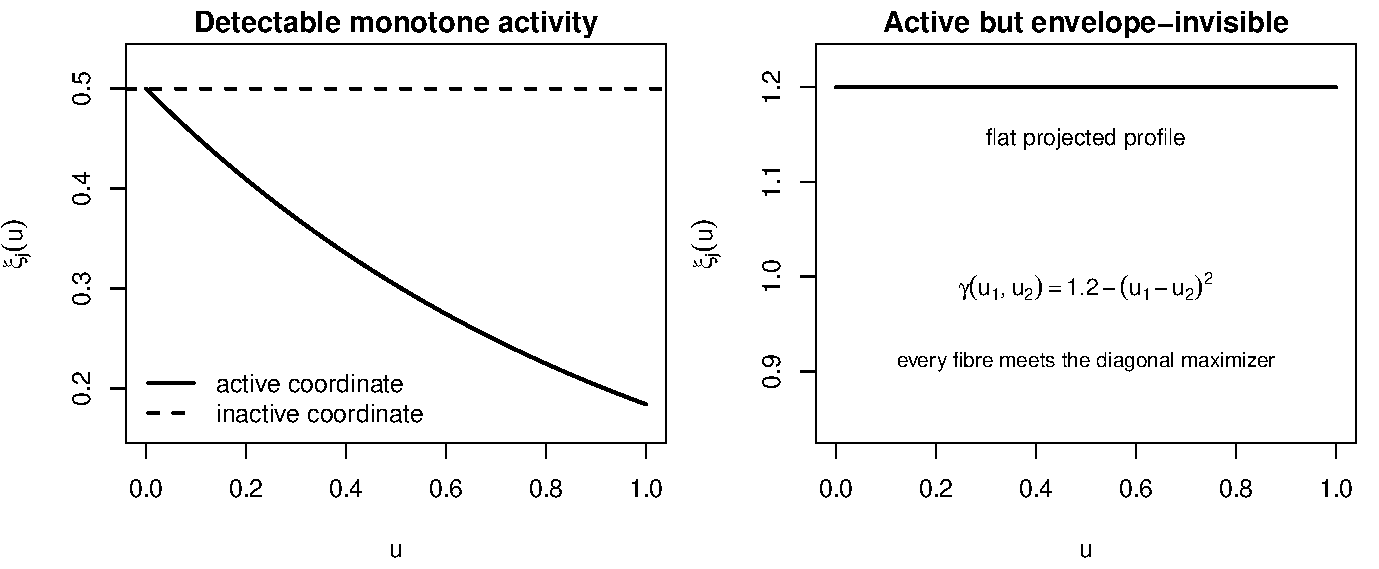
\includegraphics[width=.88\linewidth]{figures/population_profiles.pdf}
\caption{Projected envelopes. Left: a monotone active coordinate depresses
the envelope below the inactive baseline $\gmax$. Right: in the diagonal
example every fibre meets the argmax set, so the envelope of an active
coordinate stays flat.}
\label{fig:population-profiles}
\end{figure}

\begin{proposition}[Quantitative margin]\label{prop:margin}
Assume (C1)--(C2), (S), and that for some $u^\star_{\A}\in[0,1]^{\A}$ and $\nu>0$,
\[
 \gamma(u)\le\gmax-c_1\,\|u_{\A}-u^\star_{\A}\|^\nu
 \qquad\text{for all }u,
\]
for some constant $c_1>0$. Then, for $j\in\A$,
\[
 \gmax-\xi_j(u)\ge c_1\,|u-u_j^\star|^\nu,
 \qquad
 \Delta_j\ge c_1\,\E\bigl(|W-u_j^\star|^\nu\bigr),\quad
 W\sim\mathrm{Unif}(\I).
\]
For $\nu=2$ the right-hand side is at least
$c_1\{(1-2\varepsilon)^2/12+(1/2-u_j^\star)^2\}$.
\end{proposition}

Two consequences of \eqref{eq:fibre} help with examples. If
$\gamma(u)=G(\sum_{\ell\in\A}g_\ell(u_\ell))$ with $G$ strictly increasing,
then $\xi_j(u)=G(g_j(u)+\sum_{\ell\in\A,\,\ell\ne j}\max g_\ell)$, and
$\Delta_j>0$ whenever $g_j$ lies below its maximum on a subset of $\I$ of
positive measure. If $\partial_j\gamma\ge c_j>0$ throughout the cube,
arbitrary interactions are allowed and $\Delta_j\ge c_j/2$.

For the benchmark $\gamma(u)=\tfrac12\exp(-u_1-u_2-u_3-u_4)$ used in
Section~\ref{sec:simulation}, $\xi_j(u)=e^{-u}/2$ for $j\le4$ and
$\xi_j\equiv1/2$ otherwise, so $\Delta_j\approx0.186$ at
$\varepsilon=0.05$. The gap is comfortable, yet estimating $\xi_j(u)$ near
its maximum requires sample points whose remaining three active
coordinates are simultaneously small; the simulations keep population
detectability and finite-sample accessibility clearly separated.


\section{Estimation and screening theory}\label{sec:estimation}

\subsection{Empirical-rank local Hill scores}

The estimator follows the envelope construction coordinate by coordinate.
Let $R_{ij}$ be the rank of $X_{ij}$ among $X_{1j},\ldots,X_{nj}$ and
$\widehat U_{ij}=R_{ij}/(n+1)$. For $u\in\I$, form the rank window
\[
 \mathcal W_j(u)=\{i:|\widehat U_{ij}-u|\le h\},\qquad
 M_j(u)=|\mathcal W_j(u)|,\qquad
 k_j(u)=\lfloor\alpha M_j(u)\rfloor,
\]
and, writing $Y_{j,u,(1)}\le\cdots\le Y_{j,u,(M_j(u))}$ for the local order
statistics, the local Hill estimate
\begin{equation}\label{eq:hill}
 \widehat\xi_j(u)=\frac1{k_j(u)}\sum_{r=1}^{k_j(u)}
 \log\frac{Y_{j,u,(M_j(u)-r+1)}}{Y_{j,u,(M_j(u)-k_j(u))}},
\end{equation}
defined when $\alpha M_j(u)>1$. This is the local-fraction Hill statistic of
\citet[Definition~5]{gardesPodgorny2025} evaluated on one-coordinate rank
windows. The score averages the profile over the deterministic grid
$G=\{r/(n+1):r=1,\ldots,n\}\cap\I$,
\begin{equation}\label{eq:emp-score}
 \widehat\Psi_j=\frac1{|G_j^{\rm val}|}\sum_{u\in G_j^{\rm val}}\widehat\xi_j(u),
 \qquad
 G_j^{\rm val}=\{u\in G:\alpha M_j(u)>1\},
\end{equation}
Because the window counts $M_j(u)$ depend on the ranks only through
the grid position, $G_j^{\rm val}$ is the same set for every $j$, and
under the conditions of Theorem~\ref{thm:score} every grid point is
usable, so $G_j^{\rm val}=G$; the convention $\widehat\Psi_j=+\infty$
when no grid point is usable is an implementation safeguard that is
provably never triggered when $K_n\ge2$. The screened set
$\widehat\A_d$ collects the $d$ smallest scores, ties broken by a
seeded auxiliary randomization.

The two localization parameters play different roles: $h$ fixes how many
observations resemble the target rank position, roughly $2nh$ of them, and
$\alpha$ fixes how many of their largest responses enter the Hill statistic,
roughly $2n\alpha h$. Rank windows make these counts deterministic up to
boundary effects, which is what permits exact finite-sample union bounds
over a diverging number of coordinates.

\subsection{Assumptions}

Ranks displace the unobserved transforms $U_{ij}$, windows displace the
conditioning point, and the Hill statistic sees only the upper
$\alpha$-fraction of a projected distribution. The assumptions bound these
three effects uniformly over the coordinates. Throughout this section
every active coordinate is assumed detectable, $\Delta_{\min}>0$ for
every $n$, so that the conditions below are well posed. Let
$Q_j(\cdot,u)$ denote the generalized upper conditional quantile of $Y$
given $U_j=u$, $Q_j(s,u)=F_{Y|j}^{-1}(1-s^{-1}\mid u)$ with
$F^{-1}(t)=\inf\{y:F(y)\ge t\}$, and let $\tau_n=(pn)^{-2}$.

\begin{itemize}
\item[(E1)] \emph{Quantile representation and regularity of the projected
index.} For every $j\le p$ and every $u\in[0,1]$ the conditional
distribution function $F_{Y|j}(\cdot\mid u)$ is continuous, so that
$V_{ij}=1-F_{Y|j}(Y_i\mid U_{ij})$ is conditionally standard uniform and
$Y_i=Q_j(1/V_{ij},U_{ij})$ almost surely. Moreover the projected indices
are equicontinuous on $\I$, uniformly over coordinates and over $n$,
\[
 \omega_\xi(r)=\max_{j\le p}\;
 \sup_{u,v\in\I,\,|u-v|\le r}|\xi_j(u)-\xi_j(v)|
 \longrightarrow0\qquad(r\to0),
\]
and satisfy the grid-scale regularity condition
$\omega_\xi(1/n)=o(\Delta_{\min})$.
\item[(E2)] \emph{Uniform tail regularity.} Writing
$Q_j(s,u)=s^{\xi_j(u)}\ell_j(s,u)$ with $\ell_j(\cdot,u)$ slowly varying,
\[
 \max_{j\le p}\,\sup_{u\in\I}\,
 \sup_{s\ge(3\alpha)^{-1},\,t>1}
 \frac{|\log\{\ell_j(ts,u)/\ell_j(s,u)\}|}{\log t}
 \;=\;o(\Delta_{\min}).
\]
\item[(E3)] \emph{Uniform local quantile regularity.} There exists a
constant $C_0>1$ such that
\[
 \max_{j\le p}\,
 \sup_{u\in\I}\;
 \sup_{v\in[0,1],\,|u-v|\le C_0h}\;
 \sup_{w\in[\tau_n,1-\tau_n]}
 \left|\log\frac{Q_j(w^{-1},v)}{Q_j(w^{-1},u)}\right|
 \;=\;o(\Delta_{\min}).
\]
The theorems use only this one $C_0$; under \eqref{eq:rate-cond} any
$C_0>1$ suffices.
\end{itemize}

Scale nuisances enter through (E3) and not through (E2), and the
condition accommodates them. Writing
$\log Q_j(s,u)=\xi_j(u)\log s+\log\ell_j(s,u)$, the displacement over
$|v-u|\le C_0h$ splits into an index part, bounded by
$2L_\xi C_0h\log(pn)$ when $\xi_j$ is Lipschitz with constant $L_\xi$,
and a scale part which is $O(L_cC_0h)$ whenever the conditional
log-scale profile is Lipschitz in $u$ with constant $L_c$ uniform in
$n$. A covariate that shifts the conditional scale of $Y$ without
touching the index is therefore harmless in the limit, at any bounded
amplitude: both parts are $o(\Delta_{\min})$ as soon as
$h\log(pn)=o(\Delta_{\min})$. Model B1 of
Section~\ref{sec:simulation} is built to make the finite-sample
version of this statement measurable.

(E1) asks for continuity only; strict monotonicity of the conditional
distribution function is not needed, because flat pieces are visited with
probability zero. (E2) is the analogue of condition (H.4) in
\citet{gardesPodgorny2025}, normalized by $\log t$ and required only beyond
the working tail level $(3\alpha)^{-1}$; it accommodates slowly varying
factors such as $\ell(s)\asymp(\log s)^{-2}$, for which the left side is of
order $1/\log(1/\alpha)\asymp1/\log n$ when $\alpha=n^{-a}$, so gaps
$\Delta_{\min}\gg1/\log n$ are covered and smaller gaps are not. (E3)
adapts their condition (H.5): the truncation $\tau_n=(pn)^{-2}$ makes the
probability that any of the $pn$ conditional PIT variables falls below
$\tau_n$ vanish, which is the high-dimensional replacement for their
fixed-dimension truncation. Their density conditions (H.1)--(H.2)
have no counterpart here: empirical-rank windows have deterministic counts,
so no lower bound on a covariate density is required.

These conditions are stated on the projected quantiles rather than on
the primitive model, and deliberately so: projection generates slow
variation of its own, which a condition imposed upstream would have to
anticipate. If $W\sim U(0,1)$ and $\Pp(Y>y\mid W)=y^{-1/(1+W)}$
exactly, then $\Pp(Y>y)\sim4y^{-1/2}/\log y$, so even exact Pareto
conditionals produce a logarithmic factor after projection, and the
left side of (E2) is then of exact order $1/\log(1/\alpha)$. Stating
(E2) downstream measures that factor where it acts, and the resulting
requirement is mild: every gap with $\Delta_{\min}\log(1/\alpha)
\to\infty$ is covered, which for $\alpha=n^{-a}$ admits all gaps
$\Delta_{\min}\gg1/\log n$, and in particular every fixed gap.

Appendix~\ref{app:primitive} derives these conditions from primitive
assumptions. Two steps make this possible. First, the range
$w\in[\tau_n,1-\tau_n]$ in (E3) is wider than the proofs need: only the
$k+1$ largest responses of a window enter a Hill statistic, and
Lemma~\ref{lem:app-tailfreeze} shows that on the working event these are
generated by $w\le3\alpha$. Replacing (E3) by the tail-only condition
\[
 \omega_n^{\uparrow}(C_0h,\tau_n,\alpha)
 =\max_{j\le p}\sup_{u\in\I}
 \sup_{|v-u|\le C_0h}\sup_{w\in[\tau_n,3\alpha]}
 \left|\log\frac{Q_j(w^{-1},v)}{Q_j(w^{-1},u)}\right|
 =o(\Delta_{\min})
 \tag{E3$^{\uparrow}$}
\]
leaves Theorems~\ref{thm:score} and~\ref{thm:sis} unchanged, and removes
any requirement on the body of the conditional distribution. Second,
Theorem~\ref{thm:app-transfer} derives (E1), (E2) and (E3$^{\uparrow}$)
from four primitive conditions --- Lipschitz continuity and
atomlessness, a differentiable uniform tail approximation, uniform
doubling of the fibre-deficit mass for
$D_{j,u}=1/\gamma-1/\xi_j(u)$, and a horizontal coupling of the
primitive tails only --- with
\[
 \omega_\xi(1/n)=O(n^{-1}),
 \qquad
 b_n(3\alpha)=O\{1/\log(1/\alpha)\},
 \qquad
 \omega_n^{\uparrow}=O\{h\log(pn)\}.
\]
Corollary~\ref{cor:app-models} verifies the primitive conditions for the
Gaussian-copula models of Section~\ref{sec:simulation}, whose corner
margins are regularly varying with a slowly varying Gaussian factor, so
that a pure two-sided polynomial margin is neither assumed nor needed.

\subsection{Main results}

\begin{theorem}[Score concentration]\label{thm:score}
Assume (C1)--(C2), (S), (E1)--(E2), (E3$^{\uparrow}$), $\alpha\le1/3$,
$h\le1-\varepsilon$, and
\begin{equation}\label{eq:rate-cond}
 \log(pn)=o(nh^2),
 \qquad
 \log(pn)=o(n\alpha h).
\end{equation}
Then there are deterministic sequences
$a_n=O(\sqrt{\log(pn)/(n\alpha h)})$ and $\beta_n=o(\Delta_{\min})$ with
\[
 \Pp\Bigl(\max_{j\le p}\,|\widehat\Psi_j-\Psi_j|\le a_n+\beta_n\Bigr)
 \longrightarrow1;
\]
in shorthand,
$\max_{j\le p}|\widehat\Psi_j-\Psi_j|
=O_{\Pp}(\sqrt{\log(pn)/(n\alpha h)})+o(\Delta_{\min})$.
\end{theorem}

The stochastic term is the exponential-spacings fluctuation of
$O(n)$ local Hill statistics per coordinate, each built from at least
$c\,n\alpha h$ spacings, controlled simultaneously over $p$ coordinates;
$\sqrt{\log(pn)/(n\alpha h)}$ is the resulting effective-tail-sample-size
rate. The $o(\Delta_{\min})$ term collects the tail bias (E2), the spatial
bias (E3$^{\uparrow}$) evaluated at $C_0h$ --- the first condition in
\eqref{eq:rate-cond} makes the rank displacement smaller than $(C_0-1)h$,
so windows never leave the range covered by (E3$^{\uparrow}$) --- and the
quadrature
error $\omega_\xi(1/n)+O(1/n)$ from (E1).

\begin{theorem}[Sure screening]\label{thm:sis}
Assume the conditions of Theorem~\ref{thm:score} (including
$\Delta_{\min}>0$, i.e.\ every active coordinate detectable in the
sense of Proposition~\ref{prop:geometry}) and
\begin{equation}\label{eq:sis-cond}
 \log(pn)=o\bigl(n\alpha h\,\Delta_{\min}^2\bigr).
\end{equation}
Then, for every $d\ge s$,
\[
 \Pp\bigl(\A\subseteq\widehat\A_d\bigr)\longrightarrow1,
\]
and with probability tending to one every active score is smaller than
every inactive score.
\end{theorem}

\begin{corollary}[Exact recovery]\label{cor:exact}
Under the conditions of Theorem~\ref{thm:sis}, if $d=s$ then
$\Pp(\widehat\A_s=\A)\to1$.
\end{corollary}

The proofs are in Appendix~\ref{app:proofs}, supported by the auxiliary
results of Appendix~\ref{app:aux}, whose centrepiece is a finite-sample
uniform profile bound (Proposition~\ref{thm:app-rank-profile}). The
roadmap: (i) a Dvoretzky--Kiefer--Wolfowitz event per coordinate controls
all empirical-rank displacements simultaneously, contributing the
$\log(pn)=o(nh^2)$ requirement; (ii) rank windows have deterministic
local counts and pass through at most $4n+1$ membership states per
coordinate; (iii) conditionally on a covariate column, the R\'enyi
representation turns each local Hill statistic into a mean of
i.i.d.\ exponentials built from about $n\alpha h$ extremes, plus a
slowly varying remainder bounded through (E2); (iv) a union bound over
the $p(4n+1)$ states yields the $\log(pn)$ factor; (v) uniform score
accuracy below $\Delta_{\min}/2$ gives deterministic separation of
active from inactive scores. \citet[Theorem~3]{gardesPodgorny2025}
establishes the corresponding uniform consistency in fixed dimension
over a compact class of projection matrices; their covering-number
argument and density assumptions are replaced here by the rank
construction, and their result does not imply the growing-$p$ bound.

Condition \eqref{eq:sis-cond} quantifies the cost of dimension:
screening $p$ coordinates costs $\log p$ against the effective local
extreme count $n\alpha h$, deflated by the squared gap. With
$\alpha=n^{-a}$ and $h=n^{-b}/2$ and $b\le a$, dimensions up to
$\log p=o(n^{1-a-b}\Delta_{\min}^2)$ are admissible, a polynomial range
of $p$ for fixed gaps; for $b>a$ the rank-displacement condition
$\log(pn)=o(nh^2)=o(n^{1-2b})$ binds first. These ranges treat (E3$^{\uparrow}$) as given; a spatial modulus of order
$h\log(1/\tau_n)$, the natural benchmark, adds the constraint
$\log(pn)=o(n^{b}\Delta_{\min})$.


\section{Simulation study}\label{sec:simulation}

Each coordinate is scored in $O(n\log n)$ time: one sort by empirical
rank, then a sliding window over the rank grid whose local Hill statistics
are maintained by a Fenwick tree indexed by global response ranks.
Covariates are generated and processed in blocks, so the total cost is
$O(pn\log n)$ time and $O(n)$ working memory beyond the scores. At
$(n,p)=(2000,1000)$ one complete screen takes under a second on a laptop
core. Scores are sorted increasingly.

\subsection{Simulation models}\label{sec:models}

\paragraph{Family A: tail-index structure.}
Models A1, A2 and A3 share the covariate design, the slowly varying
factor, and the tail-index active set $\A_\gamma=\{1,2,3,4\}$; they
differ only in the tail-index function. Covariates are latent Gaussian
AR(1),
\[
 Z_{i1}\sim N(0,1),\qquad
 Z_{ij}=\rho Z_{i,j-1}+\sqrt{1-\rho^2}\,\epsilon_{ij},
 \qquad j=2,\ldots,p,
\]
transformed to $U_{ij}=\Phi(Z_{ij})$; the tail-index functions are
evaluated at the population transforms $U$, while the estimator sees
only $Z$ and computes its own empirical ranks. Responses are generated
by quantile inversion, $Y=V^{-\gamma(U)}\ell(1/V,\cdot)$ with
$V\sim\mathrm{Unif}(0,1)$, the mechanism of
\citet{gardesPodgorny2025}, and all three models carry their slowly
varying factor
\[
 \ell_1(s,u)=\bigl[1+\exp\{v(u)-s\}\bigr]^{-1},
 \qquad
 v(u)=2.5\,(u_5+u_6+u_7+u_8),
\]
which satisfies $\ell_1(s,u)\to1$ as $s\to\infty$: its effect vanishes
in the limit while perturbing estimation at finite tail levels. The
tail-index functions are
\begin{align*}
 \gamma_{A1}(u)&=0.5\exp\bigl(-\textstyle\sum_{j=1}^4u_j\bigr),\\
 \gamma_{A2}(u)&=0.5\exp\bigl(-0.5\textstyle\sum_{j=1}^4u_j\bigr),\\
 \gamma_{A3}(u)&=0.5\exp\bigl(-0.80\textstyle\sum_{j=1}^4u_j
 -0.20\,u_1u_2-0.15\,u_3u_4\bigr).
\end{align*}
A1 is the monotone reference, with trimmed population gap $0.186$
(Section~\ref{sec:population}). A2 weakens the signal, with gap
$0.107$. A3 adds interactions among the active coordinates while
keeping a reasonably strong signal, with gap $0.158$. All three share
the maximum $\gmax=0.5$.

\paragraph{Family B: finite-quantile scale contamination.}
Model B1 has the same tail-index function as A1,
$\gamma_{B1}=\gamma_{A1}$, hence the same active set
$\A_\gamma=\{1,2,3,4\}$ and the same gap $0.186$, and \emph{replaces}
the slowly varying factor: responses are generated with $\ell_2$ below
in place of $\ell_1$, which does not appear in B1. Let
$F_i\sim N(0,1)$ be independent of the active coordinates and of the
base AR(1) innovations, and set
\[
 \log\ell_2(s,F)=-\frac1{2s}+0.5\,\bigl\{\Phi(F)-0.5\bigr\},
\]
so the persistent scale factor lies in $[e^{-0.25},e^{0.25}]$, strictly
positive and uniformly bounded. The factor $F$ is not observed. Instead,
a block of $q_{\rm scale}=20$ proxies occupies the coordinates
$\A_{\rm scale}=\{5,\ldots,24\}$:
\[
 Z_{ij}=0.7\,F_i+\sqrt{1-0.7^2}\,\epsilon_{ij},
 \qquad j\in\A_{\rm scale},
\]
with independent standard normal proxy noises, so each proxy is
marginally standard normal, loads on $F$ at $0.7$, and the pairwise
correlation within the block is $0.49$. The B1 covariate vector is
built from a base AR(1) vector of length $p$: coordinates $1$--$4$ and
$25$--$p$ are kept from the base vector, coordinates $5$--$24$ are
replaced by the proxies, and the AR(1) chain beyond coordinate $24$
continues from the base coordinate $24$, not from the overwritten
proxy. The observed B1 covariance is therefore deliberately not AR(1)
over all coordinates; the AR(1) background is intact outside the proxy
block. Because B1 changes both the slowly varying factor and the
covariate design relative to A1, A1--B1 differences measure the joint
effect of the scale cluster and of the exchange of $\ell_1$ for
$\ell_2$, not the cluster alone.

In B1, variables $1$--$4$ determine the limiting tail index; variables
$5$--$24$ are informative about the finite conditional scale through
their common information about $F$, and do not change the limiting
exponent. A screen built on a fixed high quantile can therefore
legitimately rank the proxy cluster highly --- those variables move its
target --- even though the cluster is inactive for tail-index
screening. B1 measures the practical consequence of this target
difference. Section~\ref{sec:estimation} places the mechanism in the
theory: a bounded scale nuisance enters (E3) through a term of order
$L_ch$, which vanishes with the bandwidth, so the screen is
asymptotically immune to it; B1 measures how much sample that immunity
costs at a finite bandwidth.

\paragraph{Monte Carlo design.}
The common design is
\[
 n=2000,\qquad p\in\{500,\,1000,\,2000\},\qquad \rho=0.25,
 \qquad d=20,\qquad \varepsilon=0.05,
\]
with $1{,}000$ replications per cell and per model in the method
comparison (binomial standard errors at most $0.016$) and $200$
common-random-number replications per model in the tuning study
(standard errors at most $0.036$); Sure-$d$ denotes
$\Pp(R_{\max}\le d)$ with $R_{\max}=\max_{j\in\A_\gamma}\mathrm{rank}(j)$,
and all methods within a replication are evaluated on the same dataset.

\paragraph{Relation to the asymptotic theory.}
The simulation models instantiate the theory rather than sit beside it.
Corollary~\ref{cor:app-models} verifies the primitive conditions of
Appendix~\ref{app:primitive} for A1--A3 and B1, and shows that (E1),
(E2) and (E3$^\uparrow$) hold along the tuning sequences
$\alpha=n^{-a}$, $h=n^{-b}/2$ used throughout, with bias orders
$O(n^{-1})$, $O(1/\log n)$ and $O(n^{-b}\log n)$. The effective local
extreme count is $n\alpha h=n^{1-a-b}/2$ while the population gaps are
constants, so conditions \eqref{eq:rate-cond} and \eqref{eq:sis-cond}
reduce to $b<1/2$ and $a+b<1$: the selected $(a,b)=(0.30,0.15)$ and all
nine settings of the aggregation block satisfy them, and
Theorems~\ref{thm:score} and~\ref{thm:sis} apply. The same corollary
covers the aggregated screen, by intersecting the nine separation
events.

What the finite design does not deliver is a numerically tight bound:
at $n=2000$ and $p=1000$, $\sqrt{\log(pn)/(n\alpha h)}\approx0.67$
against $\Delta_{\min}=0.186$, and the lower endpoint entering (E2) is
only $\log\{(3\alpha)^{-1}\}\approx1.18$, so the asymptotic bounds are
not yet informative at this sample size, as is usual for rate results at
moderate $n$ (Remark~\ref{rem:app-finite}). This is why the recovery rates below are reported as
direct finite-sample evidence, and it is the practically relevant
question: the theory says the screen eventually separates active from
inactive coordinates, and the simulations measure how much sample the
separation actually needs.

\subsection{Tuning and the aggregated screen}\label{sec:tuning}

The two smoothing parameters are parameterized as
\[
 \alpha=n^{-a},\qquad h=n^{-b}/2,
\]
following the convention of \citet{gardesPodgorny2025}. Sure-20 is
evaluated for each model over the crossed grid
$a\in\{.25,.30,.35,.40,.45,.50\}$,
$b\in\{0,.05,.10,.15,.20,.30,.40\}$ at $n=2000$, $p=1000$,
$\rho=0.25$, on $200$ common-random-number replications per model: the
$200$ datasets are generated once per model and every cell of the grid
is evaluated on the same datasets, so that differences between cells
are not inflated by simulation noise. Figure~\ref{fig:tuning} shows the
four heatmaps.

The column $a=0.25$ collapses for the three A-family models (Sure-20 at
most $.125$, $.080$ and $.225$): at $\alpha=n^{-0.25}\approx0.15$ the
local Hill statistics reach into quantile regions where $\ell_1$, whose
argument $v(u)-s$ is dominated by the $U_5$--$U_8$ combination at
moderate $s$, deforms the projected distributions. B1, whose bounded
scale factor produces no such deformation, degrades only mildly there
(up to $.580$). Performance also falls toward large $a$ and large $b$
together, where the local extreme count collapses, and the degenerate
bandwidth $b=0$ is never competitive. In between, the block
$a\in\{0.30,0.35\}$, $b\in\{0.10,0.15,0.20\}$ is the best-behaved
region of the grid, but it is not a flat plateau. The four-model mean
of Sure-20 is maximized at
\[
 (a^\star,b^\star)=(0.30,\ 0.15),
\]
at $0.780$; the five other cells of the block lie between $0.718$ and
$0.773$, and the per-model values move by more than their paired
standard errors across the block --- A2, the weakest signal, falls
from $.555$ at the argmax to $.360$ at $(0.35,0.20)$. The residual
sensitivity within an otherwise good region is precisely what the
aggregated screen below is designed to absorb. We keep the argmax as
the single selected setting, with per-model Sure-20 $.935$, $.555$,
$.955$ and $.675$; because it is selected on the same $200$
replications shown in Figure~\ref{fig:tuning}, the comparison of
Section~\ref{sec:comparison} reruns everything on $1{,}000$
independent replications. At $n=2000$ the selected pair gives
$\alpha\approx0.10$, $h\approx0.16$, and about
$2n\alpha h=n^{1-a-b}\approx65$ effective local extremes per interior
window. No model is given its own tuning.

\begin{figure}[t]
\centering

\includegraphics[width=.95\linewidth]{figures/tuning_heatmaps.pdf}
\caption{Sure-20 over the $(a,b)$ tuning grid for the four models at
$n=2000$, $p=1000$, $\rho=0.25$ ($200$ common-random-number
replications per model; $\alpha=n^{-a}$, $h=n^{-b}/2$; standard errors
at most $0.036$). The dashed rectangle marks the aggregation block
$\mathcal N_9$.}
\label{fig:tuning}
\end{figure}

\paragraph{The aggregated screen.}
A single pair $(a,b)$ makes the final ranking depend entirely on one
tuning. The aggregated version of the screen uses the $3\times3$ block
of settings
\[
 \mathcal N_9=\{0.30,0.35,0.40\}\times\{0.10,0.15,0.20\},
\]
the neighbourhood of $(a^\star,b^\star)$ inside the well-behaved region
of the grid. For each setting $(a,b)\in\mathcal N_9$ and each
coordinate $j$, compute the score $\widehat\Psi_j(a,b)$ and its rank
$r_j(a,b)$ among the $p$ coordinates, ranks increasing with the score;
aggregate by
\[
 r_j^{\rm agg}=\min_{(a,b)\in\mathcal N_9}r_j(a,b),
\]
and rank the coordinates by increasing $r_j^{\rm agg}$; coordinates
sharing the same minimum are ordered by the median, then the mean, then
the maximum of their nine ranks, and any remaining ties by a seeded
auxiliary randomization. A coordinate is thus retained early whenever at least
one reasonable tuning finds evidence for it. This direction of
conservatism matches the purpose of a sure-screening first stage: false
exclusion is final, while false retention is corrected by the
second-stage multivariate analysis that the screen feeds. We make no
optimality claim for the construction; it is the procedure used in the
experiments and the application, and its effect is measured against the
single-setting screen in Section~\ref{sec:comparison}. Its cost is nine
score passes instead of one, leaving the $O(pn\log n)$ complexity
unchanged up to the constant.

The two versions are reported side by side throughout:
\emph{Tail-index SIS, selected $(a^\star,b^\star)$} uses the central
pair alone; \emph{Tail-index SIS, aggregated} uses $r_j^{\rm agg}$.

\subsection{Comparison with competing screens}\label{sec:comparison}

Six rules are compared on the same $1{,}000$ simulated datasets per
model and per dimension $p\in\{500,1000,2000\}$, at $n=2000$,
$\rho=0.25$: the two versions of the tail-index screen; the
conditional-Pickands screen of \citet{yoshidaUmezu2026}, implemented
from their equations (2)--(4) with the Epanechnikov kernel and the
tuning of their numerical work transplanted proportionally --- their
bandwidth $h=1$ on standardized covariates is kept, and their
extreme-value count is carried over as the same fraction of the sample
size, $k=\lfloor0.072\,n\rfloor$ --- on 25 equally spaced evaluation
points in $[.02,.98]$; and the quantile-adaptive SIS of \citet{heWangHong2013} at
the levels $\tau\in\{.90,.95,.99\}$, using cubic B-spline marginal
quantile regression with three degrees of freedom, identical at every
level. The competitors rank large utilities first; ours ranks small
scores first. Tables~\ref{tab:cmp500}--\ref{tab:cmp2000} report, for
each model and method, Sure-4 (exact recovery), Sure-20, and the mean
and median of the worst active rank. Both competitors run at their
authors' settings, with no counterpart of the grid search of
Section~\ref{sec:tuning}; in this respect the comparison favours the
tail screen, and Section~\ref{sec:tuning} shows how much its own
performance moves across reasonable tunings.

%% <<< tables/cmp500.tex
\begin{table}[t]
\centering
\caption{Method comparison at $n=2000$, $p=500$, $\rho=0.25$, on the same 1{,}000 replications per model. Sure-$d$ is the probability that all four tail-index-active variables rank among the $d$ smallest scores ($d=4$ is exact recovery); $\mathbb{E}(R_{\max})$ and $\mathrm{Med}(R_{\max})$ are the mean and median of the worst active rank $R_{\max}=\max_{j\in\A_\gamma}\mathrm{rank}(j)$. Standard errors of the probabilities are at most $0.016$.}
\label{tab:cmp500}
\begin{tabular}{llrrrr}
\toprule
Model & Method & Sure-4 & Sure-20 & $\mathbb{E}(R_{\max})$ & $\mathrm{Med}(R_{\max})$\\
\midrule
A1 & Tail-index SIS, selected $(a^\star,b^\star)$ & 0.849 & 0.979 & 5.7 & 4\\
 & Tail-index SIS, aggregated & 0.884 & 0.990 & 4.6 & 4\\
 & Yoshida--Umezu & 0.202 & 0.467 & 97.4 & 29\\
 & Quantile SIS ($\tau=.90$) & 0.299 & 0.894 & 11.7 & 6\\
 & Quantile SIS ($\tau=.95$) & 0.891 & 0.998 & 4.2 & 4\\
 & Quantile SIS ($\tau=.99$) & 0.125 & 0.852 & 13.0 & 9\\
\addlinespace
A2 & Tail-index SIS, selected $(a^\star,b^\star)$ & 0.256 & 0.655 & 38.2 & 9\\
 & Tail-index SIS, aggregated & 0.196 & 0.797 & 20.3 & 8\\
 & Yoshida--Umezu & 0.028 & 0.178 & 153.9 & 124\\
 & Quantile SIS ($\tau=.90$) & 0.099 & 0.597 & 33.8 & 14\\
 & Quantile SIS ($\tau=.95$) & 0.431 & 0.930 & 8.2 & 5\\
 & Quantile SIS ($\tau=.99$) & 0.005 & 0.268 & 58.5 & 37\\
\addlinespace
A3 & Tail-index SIS, selected $(a^\star,b^\star)$ & 0.775 & 0.966 & 7.0 & 4\\
 & Tail-index SIS, aggregated & 0.790 & 0.986 & 5.1 & 4\\
 & Yoshida--Umezu & 0.181 & 0.509 & 79.8 & 20\\
 & Quantile SIS ($\tau=.90$) & 0.337 & 0.915 & 10.8 & 5\\
 & Quantile SIS ($\tau=.95$) & 0.863 & 0.996 & 4.4 & 4\\
 & Quantile SIS ($\tau=.99$) & 0.077 & 0.775 & 16.8 & 11\\
\addlinespace
B1 & Tail-index SIS, selected $(a^\star,b^\star)$ & 0.308 & 0.730 & 29.8 & 7\\
 & Tail-index SIS, aggregated & 0.448 & 0.907 & 9.8 & 5\\
 & Yoshida--Umezu & 0.007 & 0.088 & 132.0 & 108\\
 & Quantile SIS ($\tau=.90$) & 0.000 & 0.017 & 24.1 & 24\\
 & Quantile SIS ($\tau=.95$) & 0.030 & 0.514 & 18.0 & 20\\
 & Quantile SIS ($\tau=.99$) & 0.037 & 0.665 & 21.3 & 15\\
\bottomrule
\end{tabular}
\end{table}
%% >>> tables/cmp500.tex
%% <<< tables/cmp1000.tex
\begin{table}[t]
\centering
\caption{Method comparison at $n=2000$, $p=1000$, $\rho=0.25$, on the same 1{,}000 replications per model. Sure-$d$ is the probability that all four tail-index-active variables rank among the $d$ smallest scores ($d=4$ is exact recovery); $\mathbb{E}(R_{\max})$ and $\mathrm{Med}(R_{\max})$ are the mean and median of the worst active rank $R_{\max}=\max_{j\in\A_\gamma}\mathrm{rank}(j)$. Standard errors of the probabilities are at most $0.016$.}
\label{tab:cmp1000}
\begin{tabular}{llrrrr}
\toprule
Model & Method & Sure-4 & Sure-20 & $\mathbb{E}(R_{\max})$ & $\mathrm{Med}(R_{\max})$\\
\midrule
A1 & Tail-index SIS, selected $(a^\star,b^\star)$ & 0.809 & 0.954 & 8.3 & 4\\
 & Tail-index SIS, aggregated & 0.823 & 0.985 & 5.1 & 4\\
 & Yoshida--Umezu & 0.179 & 0.398 & 188.1 & 58\\
 & Quantile SIS ($\tau=.90$) & 0.219 & 0.804 & 18.6 & 7\\
 & Quantile SIS ($\tau=.95$) & 0.830 & 0.997 & 4.6 & 4\\
 & Quantile SIS ($\tau=.99$) & 0.068 & 0.674 & 22.2 & 15\\
\addlinespace
A2 & Tail-index SIS, selected $(a^\star,b^\star)$ & 0.192 & 0.525 & 81.0 & 17\\
 & Tail-index SIS, aggregated & 0.151 & 0.677 & 39.5 & 10\\
 & Yoshida--Umezu & 0.021 & 0.138 & 320.1 & 256\\
 & Quantile SIS ($\tau=.90$) & 0.059 & 0.456 & 68.7 & 24\\
 & Quantile SIS ($\tau=.95$) & 0.303 & 0.873 & 14.8 & 6\\
 & Quantile SIS ($\tau=.99$) & 0.004 & 0.103 & 120.5 & 74\\
\addlinespace
A3 & Tail-index SIS, selected $(a^\star,b^\star)$ & 0.747 & 0.938 & 11.0 & 4\\
 & Tail-index SIS, aggregated & 0.706 & 0.980 & 6.7 & 4\\
 & Yoshida--Umezu & 0.176 & 0.445 & 156.8 & 34\\
 & Quantile SIS ($\tau=.90$) & 0.249 & 0.845 & 18.3 & 7\\
 & Quantile SIS ($\tau=.95$) & 0.794 & 0.992 & 4.7 & 4\\
 & Quantile SIS ($\tau=.99$) & 0.040 & 0.569 & 28.4 & 18\\
\addlinespace
B1 & Tail-index SIS, selected $(a^\star,b^\star)$ & 0.249 & 0.654 & 59.9 & 9\\
 & Tail-index SIS, aggregated & 0.368 & 0.849 & 17.0 & 5\\
 & Yoshida--Umezu & 0.004 & 0.059 & 265.5 & 206\\
 & Quantile SIS ($\tau=.90$) & 0.000 & 0.014 & 25.7 & 24\\
 & Quantile SIS ($\tau=.95$) & 0.035 & 0.489 & 18.7 & 21\\
 & Quantile SIS ($\tau=.99$) & 0.020 & 0.449 & 35.2 & 23\\
\bottomrule
\end{tabular}
\end{table}
%% >>> tables/cmp1000.tex
%% <<< tables/cmp2000.tex
\begin{table}[t]
\centering
\caption{Method comparison at $n=2000$, $p=2000$, $\rho=0.25$, on the same 1{,}000 replications per model. Sure-$d$ is the probability that all four tail-index-active variables rank among the $d$ smallest scores ($d=4$ is exact recovery); $\mathbb{E}(R_{\max})$ and $\mathrm{Med}(R_{\max})$ are the mean and median of the worst active rank $R_{\max}=\max_{j\in\A_\gamma}\mathrm{rank}(j)$. Standard errors of the probabilities are at most $0.016$.}
\label{tab:cmp2000}
\begin{tabular}{llrrrr}
\toprule
Model & Method & Sure-4 & Sure-20 & $\mathbb{E}(R_{\max})$ & $\mathrm{Med}(R_{\max})$\\
\midrule
A1 & Tail-index SIS, selected $(a^\star,b^\star)$ & 0.751 & 0.941 & 12.9 & 4\\
 & Tail-index SIS, aggregated & 0.802 & 0.981 & 6.2 & 4\\
 & Yoshida--Umezu & 0.125 & 0.305 & 432.2 & 168\\
 & Quantile SIS ($\tau=.90$) & 0.161 & 0.665 & 36.6 & 11\\
 & Quantile SIS ($\tau=.95$) & 0.758 & 0.992 & 4.8 & 4\\
 & Quantile SIS ($\tau=.99$) & 0.025 & 0.406 & 40.2 & 25\\
\addlinespace
A2 & Tail-index SIS, selected $(a^\star,b^\star)$ & 0.149 & 0.463 & 144.8 & 27\\
 & Tail-index SIS, aggregated & 0.088 & 0.561 & 76.9 & 15\\
 & Yoshida--Umezu & 0.015 & 0.084 & 640.2 & 545\\
 & Quantile SIS ($\tau=.90$) & 0.039 & 0.328 & 122.2 & 42\\
 & Quantile SIS ($\tau=.95$) & 0.234 & 0.782 & 24.7 & 7\\
 & Quantile SIS ($\tau=.99$) & 0.000 & 0.022 & 245.7 & 154\\
\addlinespace
A3 & Tail-index SIS, selected $(a^\star,b^\star)$ & 0.650 & 0.892 & 22.0 & 4\\
 & Tail-index SIS, aggregated & 0.657 & 0.963 & 8.1 & 4\\
 & Yoshida--Umezu & 0.142 & 0.379 & 336.7 & 67\\
 & Quantile SIS ($\tau=.90$) & 0.171 & 0.723 & 36.4 & 9\\
 & Quantile SIS ($\tau=.95$) & 0.698 & 0.988 & 5.4 & 4\\
 & Quantile SIS ($\tau=.99$) & 0.023 & 0.328 & 56.2 & 34\\
\addlinespace
B1 & Tail-index SIS, selected $(a^\star,b^\star)$ & 0.234 & 0.599 & 108.7 & 11\\
 & Tail-index SIS, aggregated & 0.339 & 0.805 & 22.6 & 6\\
 & Yoshida--Umezu & 0.008 & 0.057 & 494.5 & 380\\
 & Quantile SIS ($\tau=.90$) & 0.000 & 0.012 & 25.1 & 24\\
 & Quantile SIS ($\tau=.95$) & 0.038 & 0.482 & 19.0 & 21\\
 & Quantile SIS ($\tau=.99$) & 0.008 & 0.254 & 61.7 & 39\\
\bottomrule
\end{tabular}
\end{table}
%% >>> tables/cmp2000.tex
%% <<< tables/b1comp.tex
\begin{table}[t]
\centering
\caption{Model B1: average number of the twenty scale proxies among the
top 4 and top 24 positions of each ranking, by dimension (same
$1{,}000$ replications as Tables~\ref{tab:cmp500}--\ref{tab:cmp2000}).
A perfectly specific screen scores $0$; ranking the proxies first
scores $4$ and $20$.}
\label{tab:b1comp}
\begin{tabular}{lrrrrrr}
\toprule
 & \multicolumn{2}{c}{$p=500$} & \multicolumn{2}{c}{$p=1000$}
 & \multicolumn{2}{c}{$p=2000$}\\
Method & top 4 & top 24 & top 4 & top 24 & top 4 & top 24\\
\midrule
Tail-index SIS, selected $(a^\star,b^\star)$ & 0.32 & 2.73 & 0.31 & 2.30 & 0.27 & 1.72\\
Tail-index SIS, aggregated & 0.19 & 2.71 & 0.15 & 2.15 & 0.12 & 1.57\\
Yoshida--Umezu & 1.78 & 9.84 & 1.50 & 8.03 & 1.35 & 6.82\\
Quantile SIS ($\tau=.90$) & 3.82 & 20.00 & 3.82 & 20.00 & 3.79 & 20.00\\
Quantile SIS ($\tau=.95$) & 2.48 & 19.53 & 2.48 & 19.38 & 2.43 & 19.05\\
Quantile SIS ($\tau=.99$) & 0.44 & 4.53 & 0.32 & 3.06 & 0.21 & 1.85\\
\bottomrule
\end{tabular}
\end{table}
%% >>> tables/b1comp.tex

\paragraph{Sensitivity to the dimension.}
Every method degrades as $p$ grows, at very different rates, and the
mean--median contrast locates the degradation. For the selected-pair
tail screen on A1, $\E(R_{\max})$ grows from $5.7$ to $12.9$ between
$p=500$ and $p=2000$ while $\mathrm{Med}(R_{\max})$ stays at $4$: the
typical replication is unaffected, and the loss is carried by a
minority of replications in which an active coordinate falls into the
null range, where its rank scales with $p$. Aggregation compresses that
tail on every model ($\E(R_{\max})$ $4.6\to6.2$ on A1, $9.8\to22.6$
against $29.8\to108.7$ on B1, $5.1\to8.1$ against $7.0\to22.0$ on A3).
The quantile screen at $\tau=.95$ is the least dimension-sensitive rule
on the A family ($\E(R_{\max})$ $4.2\to4.8$ on A1). A2 is the most
dimension-sensitive model for every method (aggregated Sure-20
$.797\to.561$, quantile $.95$ $.930\to.782$): a weak signal loses the
most from added competition. Yoshida--Umezu degrades from a low base
throughout ($\mathrm{Med}(R_{\max})$ $29\to168$ on A1).

\paragraph{Sensitivity to the quantile level.}
On the A family the quantile screen is non-monotone in $\tau$ in every
table, in opposite directions on either side of $\tau=.95$; on B1 its
behaviour tracks its target, and Table~\ref{tab:b1comp} reports the
resulting composition of its leading positions. At $\tau=.90$ its top
four contain on average $3.8$ of the twenty scale proxies and all
twenty fill its top 24; exact recovery is zero to three decimals at
every $p$. This is coherent behaviour for a $.90$-quantile target,
which the proxies genuinely move, and it is fatal for tail-index
recovery. At $\tau=.95$ the contamination remains substantial
($2.4$--$2.5$ proxies in the top four, $19.1$--$19.5$ in the top 24,
median worst active rank $20$--$21$). At $\tau=.99$ the contamination
largely clears ($0.2$--$0.4$ proxies in the top four) because the
quantile target approaches the tail index, but the variance cost is
severe everywhere: on the A family, Sure-4 falls from $.234$--$.891$
at $\tau=.95$ to at most $.125$ at $\tau=.99$, and on B1 the level
$.99$ never reaches Sure-4 $.04$. Yoshida--Umezu, built on
Pickands-type quantile differences at its own fixed levels, is
dominated on all models and dimensions here, with $6.8$--$9.8$ of the
twenty B1 proxies in its top 24 (Table~\ref{tab:b1comp}).

\paragraph{Effect of the aggregation.}
Aggregation improves the tail screen most where failures are worst. On
B1 it lifts exact recovery from $.308/.249/.234$ to $.448/.368/.339$
across the three dimensions, divides $\E(R_{\max})$ by three to five,
and brings $\mathrm{Med}(R_{\max})$ to $5$--$6$; on A1 and A3 it moves
Sure-4 by a few points in either direction ($+3.5$, $+1.4$, $+5.1$ on
A1; $+1.5$, $-4.1$, $+0.7$ on A3) while compressing the
rank tail; Sure-20 improves in all twelve model--dimension cells. On the weak-signal A2 it
trades exact recovery ($.256\to.196$ at $p=500$,
$.149\to.088$ at $p=2000$) for substantially better inclusion
(Sure-20 $.463\to.561$ at $p=2000$; $\E(R_{\max})$ $144.8\to76.9$).
The trade is the intended one: promotion by a single reasonable tuning
occasionally admits a lucky null into the top four when the signal is
weak, and reliably rescues active coordinates from single-setting
failures further down the list. Aggregation stabilizes inclusion ---
the sure-screening objective --- rather than exact selection.

The quantile screen at a moderate level remains the strongest detector
when high quantiles and the limiting exponent share their covariates
and the signal is weak (A2); the aggregated tail screen is competitive
or better on A1 and A3, and on B1 it is the only rule whose leading
positions stay on the active set --- Sure-4 $.448/.368/.339$ and
Sure-20 $.907/.849/.805$ across the three dimensions, against at most
$.038$ and $.665$ for any fixed-quantile level, with $0.12$--$0.19$
proxies in its top four (Table~\ref{tab:b1comp}). It is degraded, not
immune: the same rule reaches Sure-4 $.884/.823/.802$ on A1, so the
scale cluster, jointly with the exchange of slowly varying factors,
costs it about forty-five points of exact recovery. For a question
about the limiting exponent itself, the two rankings are best read
side by side, as in Section~\ref{sec:realdata}: variables high on one
list and low on the other are where the two targets part ways.


\FloatBarrier

\section{Application: violent crime across U.S. communities}
\label{sec:realdata}

The analysis contains $n=1{,}993$ communities and $p=99$ candidate
predictors. Under the tuning selected in Section~\ref{sec:tuning},
$\alpha=n^{-0.3}\approx0.102$ and $h=n^{-0.15}/2\approx0.160$, so the
sample contains $n\alpha\approx204$ upper-tail observations in total and
about $2n\alpha h\approx65$ within a typical interior rank window. The
dimension is therefore comparable to the number of observations
available for local tail estimation. Unrestricted or nonparametric joint
tail modelling with $99$ covariates is poorly supported by roughly $200$
upper-tail observations, and by fewer still within any local covariate
neighbourhood; a marginal screen can rank the $99$ candidates from
exactly this information.

\subsection{Data and protocol}

The Communities and Crime data set
\citep{redmond2002}, distributed by the UCI Machine Learning Repository
in its unnormalized version, links socio-economic census attributes,
law-enforcement survey attributes and FBI crime counts for $2{,}215$ U.S.
communities. The response is the violent-crime rate per $100{,}000$
inhabitants. We keep the communities with an observed positive response
($n=1{,}993$). Preprocessing of the $124$ documented predictive
attributes is response-blind: we retain numeric predictors with fewer
than $5\%$ missing values, which removes the $22$ law-enforcement
variables reported by only $343$ communities, and with at least $100$
distinct observed values, which removes $3$ low-cardinality variables,
keeping the application close to the continuous-marginal framework of
the theory. This leaves $p=99$ continuous predictors --- demographic
composition, income and poverty, education, employment, family
structure, immigration, language, housing, and population density. The
at most one missing value per retained predictor is median-imputed, and
every method below works from the same imputed matrix.

The response is strongly right-skewed: median $374$, $99$th percentile
$2{,}943$, maximum $4{,}877$. The left panel of Figure~\ref{fig:crime}
shows the Hill curve of the response over $k\in[20,600]$ upper order
statistics; it is positive and moves slowly, between $0.283$ and
$0.374$ for $k\in[100,300]$, with value $0.328$ at the working level
$k=n\alpha=204$. The middle panel shows the Pareto QQ plot of the $600$
largest responses, approximately linear over the working range with
least-squares slope $0.27$. The gap between the QQ slope and the Hill
value at the same level is mild evidence that regular variation is only
approximate over the working range. The response exhibits a
sufficiently heavy and stable upper tail to make a tail-index analysis
plausible; neither diagnostic establishes regular variation beyond
doubt, and no single threshold carries a structural interpretation.

The screening protocol is the one fixed in Section~\ref{sec:tuning},
applied unchanged: the aggregated tail-index screen computes the score
at each of the nine settings
$\mathcal N_9=\{0.30,0.35,0.40\}\times\{0.10,0.15,0.20\}$, converts
each pass into ranks, and orders the predictors by the minimum rank
$r_j^{\rm agg}$ across the nine settings; the selected-pair screen at
$(a^\star,b^\star)=(0.30,0.15)$ is reported alongside. The two
competing screens of Section~\ref{sec:comparison} are run on the same
imputed matrix: Yoshida--Umezu at its transplanted tuning and the
quantile screen at $\tau\in\{.90,.95,.99\}$.

\subsection{Results}

Poverty and family structure dominate the aggregated ranking, and they
dominate every competing ranking as well. The two-parent household
variable \texttt{pctKids2Par} is first (per-setting ranks $1$--$4$
across the nine settings), the poverty rate \texttt{pctPoverty} second
(ranks $1$--$6$) and \texttt{pct2Par} third (ranks $1$--$5$); the two
family-structure variables are also leading variables for the quantile
screen at every level (\texttt{pctKids2Par} is first at all three
$\tau$) and for Yoshida--Umezu (ranks $3$--$7$). The related
\texttt{pctKids4w2Par} and \texttt{pct12to17w2Par} complete the
consensus block at aggregated ranks $7$--$8$. The high-quantile and
tail-index rankings share these leading predictors.

The informative disagreements are the tail-specific candidates. The
share of workers using public transportation
(\texttt{pctUsePubTrans}, aggregated rank $5$) and the farm-employment
rate (\texttt{pctWfarm}, rank $6$) rank far lower under every
fixed-quantile method: ranks $49$--$73$ for the quantile screen across
its three levels and $57$--$60$ for Yoshida--Umezu. Their low
tail-index scores are consistent with marginal variation in upper-tail
heaviness across their values, of a kind that fixed-quantile screens are
not designed to detect; Section~\ref{sec:comparison} produces the same
dissociation under controlled conditions, where the target is known.
The two variables differ in stability across the aggregation block:
\texttt{pctUsePubTrans} ranks within the top $15$ at every one of the
nine settings, while \texttt{pctWfarm} moves between $2$ and $47$
(right panel of Figure~\ref{fig:crime}). The never-married male rate
(\texttt{pctMaleNevMar}, aggregated rank $4$, per-setting ranks
$1$--$9$, quantile ranks $28$--$35$) sits between the consensus block
and the tail-specific pair. We report all three as candidate
tail-specific predictors for a second-stage analysis.

Minimum-rank aggregation is deliberately conservative: a predictor is
promoted whenever at least one tuning in the prespecified neighbourhood
ranks it highly, which suits a first-stage sure screen, where false
exclusion is more costly than retaining additional candidates.
\texttt{pctHousWOplumb} (aggregated rank $9$) and \texttt{pctLargHous}
(rank $10$) illustrate the resulting behaviour: their positions rest on
one favourable setting each (per-setting ranks $6$--$55$ and $6$--$74$;
selected-pair ranks $36$ and $46$), so their rankings are markedly more
tuning-sensitive than those of the consensus block or of the
tail-specific candidates, which hold their positions across the whole
block. The conservative screen retains them intentionally; the
per-setting ranks describe this sensitivity, and discrimination among
the retained predictors is left to the subsequent multivariate
analysis.

We do not interpret any ranking causally: the screen identifies
covariates along which the conditional tail index varies marginally,
and confounding among the $99$ predictors is certain.

\begin{figure}[t]
\centering
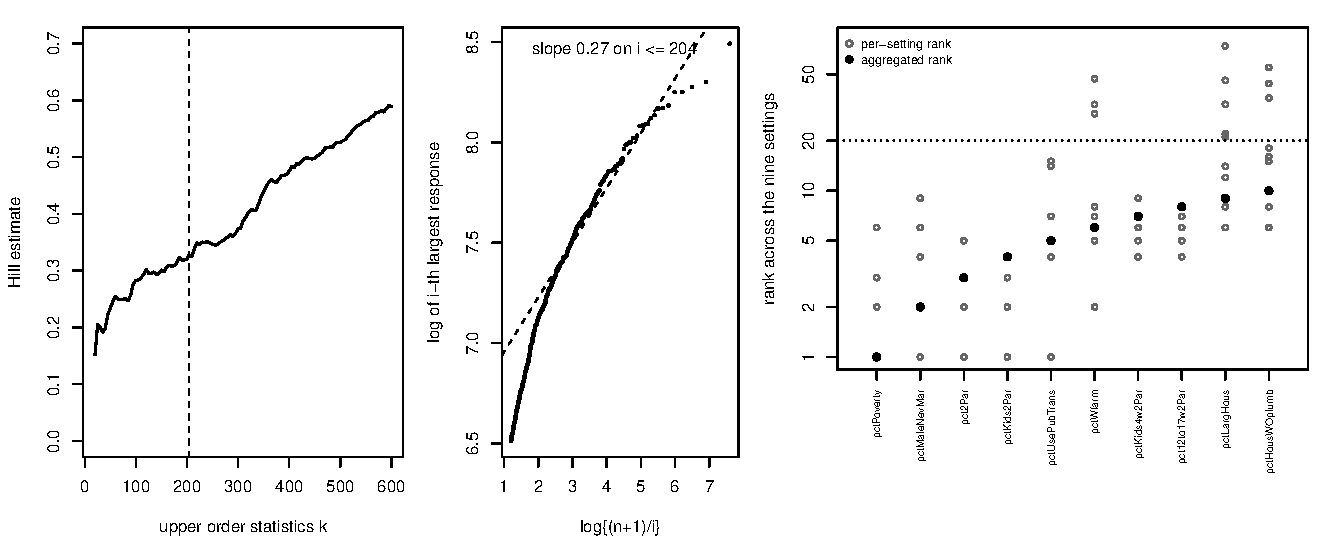
\includegraphics[width=.98\linewidth]{figures/crime_application.pdf}
\caption{Communities and Crime application ($n=1{,}993$, $p=99$,
$\alpha=n^{-0.3}$, $h=n^{-0.15}/2$). Left: Hill estimates for the
violent-crime rate; the dashed line marks the working level
$k=n\alpha=204$. Middle: Pareto QQ plot of the $600$ largest responses;
the dashed line is fitted over the working range $i\le204$. Right: for
the ten leading predictors of the aggregated screen, the nine
per-setting ranks (open circles) and the aggregated rank (filled
circles); the dotted line is the default retained size $d=20$.}
\label{fig:crime}
\end{figure}


\FloatBarrier

\section{Discussion}\label{sec:discussion}

The screen is a first stage. Its intended
pipeline reduces $p$ coordinates to a manageable $d$, after which a joint
method --- the central tail-index subspace of \citet{gardesPodgorny2025}, a
structured tail regression \citep{wangTsai2009,sasakiTaoWang2026}, or
multivariate local estimation --- can resolve interactions and correlated
neighbours among the retained variables. The two stages solve different
problems: rapid elimination of evidently irrelevant coordinates scales
to large $p$, while accurate joint tail inference does not.

The scope of a marginal screen for this target is delimited exactly
rather than assumed. An active coordinate every one of whose fibres
meets the global argmax set leaves no trace in the score, at any sample
size; Proposition~\ref{prop:geometry} characterizes this case exactly,
in terms of the argmax projections, where a signal-strength condition
would only have hidden it. Knowing the boundary is what allows a user
to tell a screen that has failed from a target that a marginal screen
cannot see, and it marks where iterative or grouped extensions, with
their own identification arguments, would be required. Two further
features of the target are worth stating in the same spirit. Projected
mixture bias is logarithmic, so (E2) covers every gap with
$\Delta_{\min}\log(1/\alpha)\to\infty$ and in particular every fixed
gap; whether gaps of the excluded order $1/\log n$ are detectable by
any estimator is a question about the target, not about this screen.
And the envelope near its maximum is estimated from observations whose
remaining active coordinates are simultaneously near their maximizing
values, so the sample cost grows with the number of active coordinates:
the weak-signal model A2 in Section~\ref{sec:simulation} measures it,
and aggregation over neighbouring tunings recovers most of it.

Appendix~\ref{app:primitive} derives the estimation conditions from
primitive assumptions that are verifiable on concrete models; what
remains is to establish whether the logarithmic projected bias, which
restricts the covered gaps to $\Delta_{\min}\log(1/\alpha)\to\infty$, is a
property of the target or of this estimator. The score functional also
invites variants: a minimum or a low quantile of the profile would
emphasize depressions confined to short intervals, at the price of new
uniformity arguments for empirical profile extrema.

In practice, tuning matters more than the theory prescribes. The tail
fraction trades Hill bias against variance; the bandwidth additionally
determines how often near-maximizing configurations of the other active
coordinates enter a window. We recommend the workflow of
Sections~\ref{sec:simulation} and~\ref{sec:realdata}: run the screen on
the block of nine neighbouring tunings and rank by the aggregated
minimum rank. The aggregation is deliberately conservative --- a
predictor is retained when at least one reasonable tuning finds
evidence for it --- which is the right direction of error for a
first-stage sure screen: false exclusion is final, while false
retention is corrected by the second-stage multivariate analysis. The
per-setting ranks describe tuning sensitivity and should accompany the
ranking as a diagnostic, not act as a second screening threshold.
Dependence deserves caution of its own: it can help, by concentrating
active configurations, or hurt, by promoting inactive neighbours, and
the direction is design-specific.

Projection turns a tail-index surface into an upper envelope. Variation
of that envelope is a scalable marginal signal for tail-index activity,
and its absence, characterized by the argmax projections, tells the
analyst exactly what a marginal screen can and cannot see.


\begin{appendix}
\section{Auxiliary results}
\label{app:aux}
\renewcommand{\theequation}{A.\arabic{equation}}
\setcounter{equation}{0}

This appendix collects the technical tools used by the proofs of
Appendix~\ref{app:proofs}: elementary probabilistic lemmas
(\ref{app:elementary}), the projection lemmas behind
Proposition~\ref{prop:projection} (\ref{app:projlem}), the deterministic
geometry of empirical-rank windows (\ref{app:rankgeom}), the local Hill
representation and the finite-sample uniform profile bound
(\ref{app:hill}), and the passage from profiles to scores, ending with a
deterministic separation lemma (\ref{app:scores}).

Throughout, the dimension is written $p=p_n$, and two auxiliary moduli
quantify the content of (E2)--(E3):
\[
 b_n(a)=\max_{j\le p}\sup_{u\in\I}\sup_{s\ge a^{-1},\,t>1}
 \frac{|\log\{\ell_j(ts,u)/\ell_j(s,u)\}|}{\log t},
 \qquad
 \omega_n(r,\tau)=\max_{j\le p}
 \sup_{u\in\I}\;
 \sup_{\substack{v\in[0,1]\\|v-u|\le r}}\;
 \sup_{w\in[\tau,1-\tau]}
 \left|\log\frac{Q_j(w^{-1},v)}{Q_j(w^{-1},u)}\right|,
\]
so that (E2) reads $b_n(3\alpha)=o(\Delta_{\min})$ and (E3) reads
$\omega_n(C_0h,\tau_n)=o(\Delta_{\min})$ with $\tau_n=(pn)^{-2}$;
$\omega_n(\cdot,\tau)$ is nondecreasing in its first argument, so (E3)
bounds $\omega_n(r,\tau_n)$ for every $r\le C_0h$.

The proofs below never use the whole range $w\in[\tau,1-\tau]$: only the
$k+1$ largest responses of a window enter a Hill statistic, and
Lemma~\ref{lem:app-tailfreeze} shows that on the working event these
correspond to $w\le3\alpha$.  We therefore also write, for
$0<\tau\le3\alpha<1$,
\begin{equation}\label{eq:omega-up}
 \omega_n^{\uparrow}(r,\tau,\alpha)=\max_{j\le p}
 \sup_{u\in\I}\;
 \sup_{\substack{v\in[0,1]\\|v-u|\le r}}\;
 \sup_{w\in[\tau,3\alpha]}
 \left|\log\frac{Q_j(w^{-1},v)}{Q_j(w^{-1},u)}\right|
 \;\le\;\omega_n(r,\tau),
\end{equation}
and record the tail-only condition
\begin{equation}\label{eq:E3up}
 \omega_n^{\uparrow}(C_0h,\tau_n,\alpha)=o(\Delta_{\min}),
 \qquad\tau_n=(pn)^{-2},
 \tag{E3$^{\uparrow}$}
\end{equation}
which is implied by (E3) and suffices everywhere below.  Every result of
this appendix and of Appendix~\ref{app:proofs} is stated with
$\omega_n^{\uparrow}$; Appendix~\ref{app:primitive} gives primitive
sufficient conditions for (E1), (E2) and (E3$^{\uparrow}$).  Put
$\delta_n=(n+1)^{-1}$,
\[
 m_n^-=\bigl\lfloor\{h+\min(h,\varepsilon)\}(n+1)\bigr\rfloor-1,
 \qquad
 K_n=\lfloor\alpha m_n^-\rfloor,
 \qquad
 S_n=4n+1.
\]
All conditional distributions are the pointwise compatible versions of
Section~\ref{sec:population}, and constants are uniform over the
triangular array.

\subsection{Elementary probabilistic lemmas}\label{app:elementary}

The first lemma transfers pointwise perturbations to order statistics, as
in \citet[Appendix, Lemma~3]{gardesPodgorny2025}.

\begin{lemma}[Sorting is sup-norm nonexpansive]\label{lem:app-sorting}
Let $a_1,\ldots,a_m$ and $b_1,\ldots,b_m$ satisfy $a_i\le b_i$ for all $i$.
Then $a_{(i)}\le b_{(i)}$ for all $i$.  Consequently
$|a_i-b_i|\le\epsilon$ for all $i$ implies
$|a_{(i)}-b_{(i)}|\le\epsilon$ for all $i$.
\end{lemma}

\begin{proof}
Fix $i$.  At least $m-i+1$ indices $r$ satisfy $a_r\ge a_{(i)}$, and for
each such $r$, $b_r\ge a_r\ge a_{(i)}$; hence $b_{(i)}\ge a_{(i)}$.  For
the second claim apply the first to $(a_i-\epsilon,b_i)$ and
$(b_i-\epsilon,a_i)$.
\end{proof}

\begin{lemma}[Chernoff bound for exponential means]\label{lem:app-chernoff}
Let $L_k$ be the mean of $k$ i.i.d.\ standard exponentials.  For
$0<t\le1$,
$\Pp(|L_k-1|>t)\le2e^{-kt^2/4}$.
\end{lemma}

\begin{proof}
Markov's inequality applied to $e^{\lambda kL_k}$, optimized at
$\lambda=t/(1+t)$, gives
$\Pp(L_k>1+t)\le e^{-k\{t-\log(1+t)\}}$.  The function
$\varphi(t)=t-\log(1+t)-t^2/4$ has $\varphi(0)=0$ and
\[
 \varphi'(t)=1-\frac1{1+t}-\frac t2=\frac{t(1-t)}{2(1+t)}\ge0
 \quad\text{on }[0,1],
\]
so $t-\log(1+t)\ge t^2/4$ on $(0,1]$.  For the lower tail,
$\Pp(L_k<1-t)\le e^{-k\{-t-\log(1-t)\}}$ and
$-t-\log(1-t)\ge t^2/2\ge t^2/4$.
\end{proof}

\begin{lemma}[Threshold order statistic of uniforms]\label{lem:app-threshold}
Let $V_{(1)}<\cdots<V_{(m)}$ be the order statistics of $m$ i.i.d.\
standard uniforms, $0<\alpha\le1/3$ and
$k=\lfloor\alpha m\rfloor\ge1$.  Then
$\Pp\{V_{(k+1)}>3\alpha\}\le e^{-(k+1)/4}$.
\end{lemma}

\begin{proof}
If $3\alpha\ge1$ the probability is zero.  Otherwise
$\{V_{(k+1)}>3\alpha\}=\{N\le k\}$ with
$N\sim\mathrm{Bin}(m,3\alpha)$ and mean $\mu=3\alpha m\ge3k$.  The
multiplicative Chernoff bound
$\Pp\{N\le(1-\delta)\mu\}\le e^{-\delta^2\mu/2}$
\citep[Section~2.2]{boucheronLugosiMassart2013} with $\delta=2/3$ gives
$\Pp(N\le\mu/3)\le e^{-2\mu/9}\le e^{-2k/3}\le e^{-(k+1)/4}$, the last
step because $8k\ge3(k+1)$ for $k\ge1$.
\end{proof}

\subsection{Projection lemmas}\label{app:projlem}

Let $\mathcal G\subseteq\sigma(U)$, $T=\gamma(U)$, and
$\xi=\esssup(T\mid\mathcal G)$, the smallest $\mathcal G$-measurable random
variable dominating $T$ almost surely.

\begin{lemma}[Uniform remainder replacement]\label{lem:app-remainder}
Define $N(y)=\E\{c(U)y^{-1/T}\mid\mathcal G\}$.  Under (C1)--(C2), almost
surely,
\begin{equation}
 \left|\frac{\Pp(Y>y\mid\mathcal G)}{N(y)}-1\right|
 \le\rho(y):=\sup_u\left|\frac{L(y,u)}{c(u)}-1\right|\longrightarrow0.
 \label{eq:A1}
\end{equation}
\end{lemma}

\begin{proof}
By the tower property,
$\Pp(Y>y\mid\mathcal G)=\E\{y^{-1/T}L(y,U)\mid\mathcal G\}$.  Writing
$L(y,U)=c(U)\{1+r(y,U)\}$ with $|r(y,U)|\le\rho(y)$,
\[
 |\Pp(Y>y\mid\mathcal G)-N(y)|
 =\bigl|\E\{c(U)y^{-1/T}r(y,U)\mid\mathcal G\}\bigr|
 \le\rho(y)N(y),
\]
and $\rho(y)\to0$ is (C2).
\end{proof}

The next lemma is the point at which the argument departs from the proof
of Proposition~1 in \citet{gardesPodgorny2025}: their condition (C.1)
assumes the law of $\gamma(X)$ absolutely continuous, which identifies
$\{\gamma>t\}$ with $\{\gamma\ge t\}$ in their computation.  The tilting
argument below needs no such assumption and allows purely atomic
conditional laws of $T$ --- the relevant case for inactive coordinates
and constant-index null models.

\begin{lemma}[Tilted-measure concentration]\label{lem:app-tilt}
For $y>1$ define the random probability measure
\[
 K_y^\star(A)=
 \frac{\E\{c(U)y^{-1/T}\mathbf 1_{\{T\in A\}}\mid\mathcal G\}}{N(y)},
 \qquad A\in\mathcal B([\underline\gamma,\Gamma]).
\]
On a common probability-one event, $K_y^\star\Rightarrow\delta_\xi$ weakly
as $y\to\infty$.
\end{lemma}

\begin{proof}
Since $K_y^\star\{T>\xi+\delta\}=0$ for every $\delta>0$ by definition of
$\xi$, it suffices to prove, for fixed
$\delta\in(0,\underline\gamma)$,
\begin{equation}
 K_y^\star\{T\le\xi-\delta\}\longrightarrow0\qquad\text{almost surely.}
 \label{eq:A2}
\end{equation}
Split by the $\mathcal G$-measurable event
$G_\delta=\{\xi\ge\underline\gamma+\delta\}$.  On $G_\delta^c$,
$\xi-\delta<\underline\gamma\le T$, so $\{T\le\xi-\delta\}$ is empty and
\eqref{eq:A2} is trivial.  On $G_\delta$, set $r=\xi-\delta$,
$s=\xi-\delta/2$ and $\pi=\Pp(T>s\mid\mathcal G)$.  Then $\pi>0$ almost
surely on $G_\delta$: otherwise
$\xi'=\xi-(\delta/2)\mathbf 1_{G_\delta\cap\{\pi=0\}}$ would be a
$\mathcal G$-measurable almost-sure upper bound for $T$, strictly smaller
than $\xi$ with positive probability, contradicting minimality of the
conditional essential supremum.  Bounding numerator and denominator
separately, using only $c_-\le c\le c_+$ and monotonicity of
$g\mapsto y^{-1/g}$,
\[
 K_y^\star\{T\le r\}
 \le\frac{c_+y^{-1/r}}{c_-\pi y^{-1/s}}
 =\frac{c_+}{c_-\pi}\,y^{-(1/r-1/s)}\longrightarrow0.
\]
A rational sequence $\delta\downarrow0$ and a countable intersection give
a common probability-one event.
\end{proof}

\begin{lemma}[Continuity of the envelope]\label{lem:app-envelope-cont}
Under (C1) and (S), so that $\xi_j(u)$ equals the fibre maximum
$\max_v\gamma(u,v)$, each $\xi_j$ is continuous on $[0,1]$, with
modulus bounded by the modulus of continuity of $\gamma$.
\end{lemma}

\begin{proof}
$\gamma$ is uniformly continuous on the compact cube; if
$|u-u'|\le\delta$ then $|\gamma(u,v)-\gamma(u',v)|\le\varpi(\delta)$ for
every $v$, and taking maxima preserves the bound.
\end{proof}

\subsection{Empirical-rank geometry}\label{app:rankgeom}

The three lemmas of this subsection are purely deterministic or
rank-based; no property of the response enters.  They replace the
covariate-density conditions (H.1)--(H.2) of
\citet{gardesPodgorny2025} in the present empirical-rank setting.

\begin{lemma}[Rank displacement]\label{lem:app-dkw}
Let $\widehat U_{ij}=R_{ij}/(n+1)$ and
\[
 D_n(\eta)=\Bigl\{\max_{j\le p}\max_{i\le n}
 |U_{ij}-\widehat U_{ij}|\le\eta+\delta_n\Bigr\}.
\]
Then $\Pp\{D_n(\eta)^c\}\le2pe^{-2n\eta^2}$.
\end{lemma}

\begin{proof}
Fix $j$ and let $F_{n,j}$ be the empirical distribution function of the
$U_{ij}$, $i\le n$.  By the Dvoretzky--Kiefer--Wolfowitz inequality with
Massart's constant \citep{massart1990},
$\sup_t|F_{n,j}(t)-t|\le\eta$ outside probability
$2e^{-2n\eta^2}$.  On that event, continuity gives
$F_{n,j}(U_{(r)j})=r/n$, hence $|U_{(r)j}-r/n|\le\eta$ and
\[
 |U_{(r)j}-r/(n+1)|\le\eta+\frac{r}{n(n+1)}\le\eta+\delta_n
\]
for every rank $r$ simultaneously.  A union bound over $j$ finishes; no
union over ranks is needed.
\end{proof}

\begin{lemma}[Deterministic window counts]\label{lem:app-counts}
For every $j$, every realization and every $u\in\I$,
$M_j(u)\ge m_n^-$ and $k_j(u)\ge K_n$; moreover $M_j(u)$ is a nonrandom
function of $u$.
\end{lemma}

\begin{proof}
The ranks form a permutation of $1,\ldots,n$, so
$M_j(u)=\#\{r\in\{1,\ldots,n\}:|r/(n+1)-u|\le h\}$, a deterministic
function of $u$: the number of integers in
$[x(u),y(u)]$ with $x(u)=\max\{(u-h)(n+1),1\}$ and
$y(u)=\min\{(u+h)(n+1),n\}$.  Fix $u\in\I$ and write
$m^-=m_n^-=\lfloor\{h+\min(h,\varepsilon)\}(n+1)\rfloor-1$; note
$h+\min(h,\varepsilon)\le\min(2h,\,h+\varepsilon)$.  Four cases.

If neither endpoint is clipped, the interval has length $2h(n+1)$ and
contains at least $\lfloor2h(n+1)\rfloor-1\ge m^-$ integers.

If only the left endpoint is clipped, then $x(u)=1$ and the count is
$\lfloor y(u)\rfloor$.  Either $y(u)=(u+h)(n+1)\ge(\varepsilon+h)(n+1)$,
so the count is at least
$\lfloor(h+\varepsilon)(n+1)\rfloor\ge m^-+1$; or $y(u)=n$ and the count
is $n\ge\lfloor(h+\varepsilon)(n+1)\rfloor-1\ge m^-$, using
$h\le1-\varepsilon$, i.e.\ $(h+\varepsilon)(n+1)\le n+1$.

If only the right endpoint is clipped, then $y(u)=n$ and the count is
$n-\lceil x(u)\rceil+1\ge n-x(u)\ge n-(1-\varepsilon-h)(n+1)
=(h+\varepsilon)(n+1)-1$, hence at least
$\lceil(h+\varepsilon)(n+1)\rceil-1\ge m^-$.

If both endpoints are clipped, the count is $n$, which is at least
$m^-$ as in the second case.  In every case $M_j(u)\ge m^-$, and
$k_j(u)=\lfloor\alpha M_j(u)\rfloor\ge\lfloor\alpha m_n^-\rfloor=K_n$.
\end{proof}

\begin{lemma}[Finite-state structure]\label{lem:app-states}
For fixed $j$ and fixed ranks, $u\mapsto\mathcal W_j(u)$ takes at most
$S_n=4n+1$ distinct values on $[0,1]$.
\end{lemma}

\begin{proof}
The membership indicator of observation $i$ changes only at
$\widehat U_{ij}\pm h$: at most $2n$ breakpoints, hence at most $2n+1$
constancy intervals plus the $2n$ breakpoint states.
\end{proof}

\begin{lemma}[Local extreme count]\label{lem:app-kn}
If $nh\ge4$ and $\alpha m_n^-\ge2$, then $m_n^-\ge nh/2$ and
\[
 \frac{n\alpha h}{4}\;\le\;K_n\;\le\;2n\alpha h+1 .
\]
\end{lemma}

\begin{proof}
$m_n^-\ge\lfloor h(n+1)\rfloor-1\ge h n-2\ge nh/2$ for $nh\ge4$, and
$K_n=\lfloor\alpha m_n^-\rfloor\ge\alpha m_n^-/2\ge n\alpha h/4$ when
$\alpha m_n^-\ge2$ (since $\lfloor x\rfloor\ge x/2$ for $x\ge2$).  For the upper bound, $m_n^-\le2h(n+1)-1\le2hn+2h-1\le2hn+1$, so
$K_n\le\alpha m_n^-\le2n\alpha h+\alpha\le2n\alpha h+1$.
\end{proof}

The rate conditions \eqref{eq:rate-cond} force $nh\to\infty$ and
$K_n\to\infty$, so Lemma~\ref{lem:app-kn} applies for $n$ large; it is
the only conversion between $K_n$ and $n\alpha h$ used in
Appendix~\ref{app:proofs}.

\subsection{Local Hill representation and uniform profile control}
\label{app:hill}

The scheme parallels the proof of Theorem~3 in
\citet{gardesPodgorny2025} --- oscillation control,
exponential-spacings representation, slowly varying remainder --- with
the covering net over their compact matrix class replaced by exact union
bounds over $p$ coordinates and $S_n$ window states.

\begin{lemma}[Conditional PIT and R\'enyi representation]\label{lem:app-pit}
Fix $j$ and condition on the column $\bm U_j=(U_{1j},\ldots,U_{nj})$.
Under (E1):
\begin{enumerate}
\item $V_{ij}=1-F_{Y|j}(Y_i\mid U_{ij})$, $i\le n$, are i.i.d.\ standard
uniform, and $Y_i=Q_j(1/V_{ij},U_{ij})$ almost surely;
\item for any index set $\mathcal W$ of size $m$, deterministic given
$\bm U_j$, with $V_{(1)}<\cdots<V_{(m)}$ the ordered PIT values of its
members and $k=\lfloor\alpha m\rfloor$,
\[
 L_k=\frac1k\sum_{r=1}^k\log\frac{V_{(k+1)}}{V_{(r)}}
\]
is distributed as the mean of $k$ i.i.d.\ standard exponentials,
independent of $V_{(k+1)}$.
\end{enumerate}
\end{lemma}

\begin{proof}
(i) Given $\bm U_j$, the pairs $(U_{ij},Y_i)$ are independent in $i$ and
$Y_i$ has continuous conditional distribution function
$F_{Y|j}(\cdot\mid U_{ij})$, so $V_{ij}$ is standard uniform.  For the
representation, $Q_j(1/V_{ij},U_{ij})=F_{Y|j}^{-1}(F_{Y|j}(Y_i\mid
U_{ij})\mid U_{ij})\le Y_i$ always, with strict inequality only when
$Y_i$ lies in the interior of an interval on which
$F_{Y|j}(\cdot\mid U_{ij})$ is constant; each such interval has
conditional probability zero and there are countably many, so the
representation holds almost surely.  Strict monotonicity is not needed.
Conditioning on the whole column, rather than on window counts as in
\citet[Appendix, Lemma~4]{gardesPodgorny2025}, makes the window sets
deterministic (Lemma~\ref{lem:app-counts}); only coordinate $j$ is
conditioned on, and no independence across coordinates is used.

(ii) With $W_i=-\log V_i$ standard exponentials and order statistics
$W_{(1)}<\cdots<W_{(m)}$, $W_{(m-r+1)}=-\log V_{(r)}$, Abel summation
gives
\[
 kL_k=\sum_{r=1}^k\{W_{(m-r+1)}-W_{(m-k)}\}
 =\sum_{i=1}^k i\,\{W_{(m-i+1)}-W_{(m-i)}\},
\]
and by the R\'enyi representation of exponential order statistics
\citep{renyi1953} the normalized top spacings
$i\{W_{(m-i+1)}-W_{(m-i)}\}$, $i\le k$, are i.i.d.\ standard exponential
and independent of $W_{(m-k)}$, hence of $V_{(k+1)}$.
\end{proof}

The next lemma is the reason no control of central quantiles is needed:
only the $k+1$ largest responses enter a Hill statistic, and on the
working event they are generated by PIT values below $3\alpha$.

\begin{lemma}[Tail-only freezing of the upper order statistics]
\label{lem:app-tailfreeze}
Fix $0<\tau\le3\alpha<1$ and a window state $\mathcal W$ of size $m$
realized at $u$, with $k=\lfloor\alpha m\rfloor$.  Write
$Z_i=\log Q_j(V_{ij}^{-1},U_{ij})$ and
$\check Z_i=\log Q_j(V_{ij}^{-1},u)$, and let $Z_{[1]}\ge\cdots\ge Z_{[m]}$
and $\check Z_{[1]}\ge\cdots\ge\check Z_{[m]}$ be the descending order
statistics.  On the event $\{\min_{i\in\mathcal W}V_{ij}\ge\tau\}\cap
\{V_{(k+1)}\le q:=3\alpha\}$, if every member satisfies
$|U_{ij}-u|\le r$, then
\begin{equation}\label{eq:tailfreeze}
 \max_{1\le s\le k+1}\bigl|Z_{[s]}-\check Z_{[s]}\bigr|
 \le\omega:=\omega_n^{\uparrow}(r,\tau,\alpha),
\end{equation}
and consequently the corresponding Hill statistics satisfy
$|H-\check H|\le2\omega$.
\end{lemma}

\begin{proof}
Let $T=\{i\in\mathcal W:V_{ij}\le q\}$.  For $i\in T$ we have
$V_{ij}\in[\tau,q]$, so \eqref{eq:omega-up} gives
$|Z_i-\check Z_i|\le\omega$.  For $i\notin T$, monotonicity of
$s\mapsto Q_j(s,\cdot)$ gives
\begin{equation}\label{eq:tailfreeze-out}
 Z_i\le\log Q_j(q^{-1},U_{ij})\le\log Q_j(q^{-1},u)+\omega
 \le\check Z_{[k+1]}+\omega,
\end{equation}
the last inequality because $V_{(k+1)}\le q$ forces at least $k+1$ members
to have $\check Z_i\ge\log Q_j(q^{-1},u)$.  Fix $s\le k+1$.  The indices
carrying the $s$ smallest PIT values lie in $T$, and their frozen values
are at least $\check Z_{[s]}$ by monotonicity of $Q_j(\cdot,u)$; their
actual values are therefore at least $\check Z_{[s]}-\omega$, whence
$Z_{[s]}\ge\check Z_{[s]}-\omega$.  Conversely at most $s-1$ indices of
$T$ have $\check Z_i>\check Z_{[s]}$; every remaining index of $T$ has
$Z_i\le\check Z_{[s]}+\omega$, while \eqref{eq:tailfreeze-out} and
$\check Z_{[k+1]}\le\check Z_{[s]}$ give the same bound outside $T$.
Hence $Z_{[s]}\le\check Z_{[s]}+\omega$, proving
\eqref{eq:tailfreeze}.  The Hill statistic is an average of differences
of the first $k$ order statistics and the $(k+1)$st, so its perturbation
is at most $2\omega$.
\end{proof}

\begin{lemma}[Frozen-location Hill expansion]\label{lem:app-hill}
Fix $j$, condition on $\bm U_j$, and fix a window state $\mathcal W$ of
size $m$ realized at $u\in\I$, with $k=\lfloor\alpha m\rfloor$ and Hill
statistic $H$.  On the event $D_n(\eta)$ intersected with
$\{V_{ij}\ge\tau\ \forall i\}$ and $\{V_{(k+1)}\le3\alpha\}$,
\begin{equation}
 |H-\xi_j(u)|
 \le2\omega_n^{\uparrow}(h+\eta+\delta_n,\tau,\alpha)
 +\xi_j(u)|L_k-1|+b_n(3\alpha)L_k.
 \label{eq:A3app}
\end{equation}
\end{lemma}

\begin{proof}
\emph{Spatial freezing.}  Each $i\in\mathcal W$ has
$|\widehat U_{ij}-u|\le h$, hence $|U_{ij}-u|\le r_n:=h+\eta+\delta_n$ on
$D_n(\eta)$.  Lemma~\ref{lem:app-tailfreeze}, applied with $r=r_n$, gives
$|H-\check H|\le2\omega_n^{\uparrow}(r_n,\tau,\alpha)$, where $\check H$
is the Hill statistic of the frozen responses
$\check Y_i=Q_j(1/V_{ij},u)$.

\emph{Exact decomposition.}  Since $s\mapsto Q_j(s,u)$ is nondecreasing,
$\check Y_{(m-r+1)}=Q_j(1/V_{(r)},u)$, and
$\log Q_j(s,u)=\xi_j(u)\log s+\log\ell_j(s,u)$ yields
\[
 \check H=\xi_j(u)L_k+R,
 \qquad
 R=\frac1k\sum_{r=1}^k
 \log\frac{\ell_j(1/V_{(r)},u)}{\ell_j(1/V_{(k+1)},u)}.
\]

\emph{Remainder.}  On $\{V_{(k+1)}\le3\alpha\}$, each ratio is
$\ell_j(ts,u)/\ell_j(s,u)$ with $s=1/V_{(k+1)}\ge(3\alpha)^{-1}$ and
$t=V_{(k+1)}/V_{(r)}>1$, so
$|\log(\cdot)|\le b_n(3\alpha)\log(V_{(k+1)}/V_{(r)})$; averaging gives
$|R|\le b_n(3\alpha)L_k$.
\end{proof}

The decomposition behind \eqref{eq:A3app} is the shape of the whole
argument:
\[
 \widehat\xi_j(u)-\xi_j(u)
 =\text{rank/spatial error}
 +\text{exponential fluctuation}
 +\text{tail remainder}.
\]

\begin{proposition}[Finite-sample uniform profile bound]
\label{thm:app-rank-profile}
Assume (C1)--(C2), (S), the structural part of (E1) (continuity of
every $F_{Y|j}(\cdot\mid u)$, hence the quantile representation), that
$b_n(3\alpha)$ and $\omega_n^{\uparrow}(\cdot,\cdot,\cdot)$ are finite,
$0<h\le1-\varepsilon$, $0<\alpha\le1/3$, and $K_n\ge2$.  For every
$\eta>0$, $0<t\le1$, $0<\tau\le3\alpha$,
\begin{align}
&\Pp\left\{\max_{j\le p}\sup_{u\in\I}
 |\widehat\xi_j(u)-\xi_j(u)|
 >2\omega_n^{\uparrow}(h+\eta+\delta_n,\tau,\alpha)
 +\Gamma t+(1+t)b_n(3\alpha)\right\}
 \nonumber\\
&\qquad\le
 \underbrace{2pe^{-2n\eta^2}}_{\text{ranks}}
 +\underbrace{pn\tau}_{\text{PIT truncation}}
 +\underbrace{2pS_ne^{-K_nt^2/4}}_{\text{spacings}}
 +\underbrace{pS_ne^{-(K_n+1)/4}}_{\text{threshold}}.
 \label{eq:A4app}
\end{align}
\end{proposition}

\begin{proof}
Call a window state \emph{admissible} for coordinate $j$ if it equals
$\mathcal W_j(u)$ for some $u\in\I$; by
Lemmas~\ref{lem:app-counts} and~\ref{lem:app-states} there are at most
$S_n$ admissible states per coordinate and each has
$k\ge K_n\ge2$, so $L_k$ and $V_{(k+1)}$ are well defined on every one of
them.  (States realized only outside $\I$ may have smaller windows; they
are not needed.)  Define the exceptional events
$T_1=D_n(\eta)^c$;
$T_2=\{\exists\,i,j:V_{ij}<\tau\}$;
$T_3=\{\exists\,j,\text{ admissible state }\mathcal W:|L_k-1|>t\}$;
$T_4=\{\exists\,j,\text{ admissible state }\mathcal W:
V_{(k+1)}>3\alpha\}$.

Outside $T_1\cup T_2\cup T_3\cup T_4$, fix $j$ and $u\in\I$: the realized
window is an admissible state, and
Lemma~\ref{lem:app-hill} with $\xi_j\le\Gamma$, $|L_k-1|\le t$,
$L_k\le1+t$ gives the displayed deviation bound; the modulus
$\omega_n^{\uparrow}(h+\eta+\delta_n,\tau,\alpha)$ covers every selected
observation because its definition allows the displaced point
$v=U_{ij}$ to range over all of $[0,1]$, and, by
Lemma~\ref{lem:app-tailfreeze}, only PIT values in $[\tau,3\alpha]$ are
involved.  The upper truncation $V_{ij}\le1-\tau$ is never used.

Probabilities: $\Pp(T_1)\le2pe^{-2n\eta^2}$ is
Lemma~\ref{lem:app-dkw}; $\Pp(T_2)\le pn\tau$ since each $V_{ij}$ is
uniform.  For $T_3$, $T_4$, condition on $\bm U_j$; the admissible states
are then deterministic with $k\ge K_n$,
Lemma~\ref{lem:app-pit} applies to each, and
Lemmas~\ref{lem:app-chernoff} and~\ref{lem:app-threshold} give conditional
bounds $2e^{-kt^2/4}\le2e^{-K_nt^2/4}$ and
$e^{-(k+1)/4}\le e^{-(K_n+1)/4}$, both decreasing in $k$.  A union bound
over the at most $pS_n$ admissible states and
integration over $\bm U_j$ complete the proof; overlapping states and
dependent coordinates cost nothing beyond the union bound.
\end{proof}

\subsection{From profiles to scores}\label{app:scores}

Recall the score grid $G=\{r\delta_n:r=1,\ldots,n\}\cap\I$, of size
$L_n=|G|$, and that $K_n\ge2$ makes every grid point usable, so
$\widehat\Psi_j=L_n^{-1}\sum_{u\in G}\widehat\xi_j(u)$.

\begin{lemma}[Quadrature]\label{lem:app-quadrature}
If $L_n\ge1$, then for every $j$,
\begin{equation}
 \Bigl|L_n^{-1}\sum_{u\in G}\xi_j(u)-\Psi_j\Bigr|
 \le q_n:=\omega_\xi(\delta_n)+\frac{4\Gamma\delta_n}{1-2\varepsilon}.
 \label{eq:A5app}
\end{equation}
\end{lemma}

\begin{proof}
Write the grid points $u_1<\cdots<u_{L_n}$, consecutive multiples of
$\delta_n$.  If $L_n=1$, then $\I$ contains a single multiple of
$\delta_n$, which forces $|\I|<2\delta_n$; the left side is at most
$\Gamma$, while $4\Gamma\delta_n/|\I|>2\Gamma$, so \eqref{eq:A5app}
holds trivially.  Assume $L_n\ge2$ and partition $\I$
exactly: $C_1=[\varepsilon,u_1+\delta_n/2]$,
$C_{L_n}=[u_{L_n}-\delta_n/2,1-\varepsilon]$, and
$C_r=[u_r-\delta_n/2,u_r+\delta_n/2]$ otherwise.  Interior cells have
length $\delta_n$, boundary cells length in $[\delta_n/2,3\delta_n/2)$,
and every point of $C_r$ is within $\delta_n$ of $u_r$.  Then
\[
 \Bigl|\frac1{L_n}\sum_r\xi_j(u_r)-\frac1{|\I|}\int_{\I}\xi_j\Bigr|
 \le\frac1{|\I|}\sum_r\int_{C_r}|\xi_j-\xi_j(u_r)|
 +\Gamma\sum_r\Bigl|\frac{\lambda(C_r)}{|\I|}-\frac1{L_n}\Bigr|.
\]
The first term is at most $\omega_\xi(\delta_n)$.  For the second, both
weight vectors sum to one;
$|\I|=\sum_r\lambda(C_r)\in[(L_n-1)\delta_n,(L_n+1)\delta_n]$ gives
$||\I|/L_n-\delta_n|\le\delta_n/L_n$, so interior cells contribute at most
$\delta_n$ in total and the two boundary cells at most
$\delta_n/2+\delta_n/L_n\le\delta_n$ each; the sum is at most $3\delta_n$,
and the second term is at most $3\Gamma\delta_n/|\I|\le
4\Gamma\delta_n/|\I|$.
\end{proof}

\begin{proposition}[Finite-sample score bound]\label{thm:app-score}
Under the conditions of Proposition~\ref{thm:app-rank-profile} (with in
addition $\omega_\xi(\delta_n)<\infty$) and $L_n\ge1$, for every
$\eta>0$, $0<t\le1$, $0<\tau<1/2$,
\begin{align}
 \Pp\Bigl\{\max_{j\le p}|\widehat\Psi_j-\Psi_j|
 >B_n(\eta,t,\tau)+q_n\Bigr\}
 \le
 2pe^{-2n\eta^2}+pn\tau+2pS_ne^{-K_nt^2/4}+pS_ne^{-(K_n+1)/4},
 \label{eq:A6app}
\end{align}
where
$B_n(\eta,t,\tau)=2\omega_n^{\uparrow}(h+\eta+\delta_n,\tau,\alpha)+\Gamma t
+(1+t)b_n(3\alpha)$.
\end{proposition}

\begin{proof}
Pathwise,
\[
 |\widehat\Psi_j-\Psi_j|
 \le\sup_{u\in\I}|\widehat\xi_j(u)-\xi_j(u)|
 +\Bigl|L_n^{-1}\sum_{u\in G}\xi_j(u)-\Psi_j\Bigr|,
\]
and Lemma~\ref{lem:app-quadrature} bounds the second term by $q_n$ on
every sample path; reusing the same observations for estimation and
averaging therefore costs no extra probability.
Proposition~\ref{thm:app-rank-profile} gives \eqref{eq:A6app}.
\end{proof}

\begin{lemma}[Deterministic score separation]\label{lem:app-separation}
Suppose $\Delta_{\min}>0$ and, on some event,
\[
 \max_{j\le p}\,|\widehat\Psi_j-\Psi_j|<\frac{\Delta_{\min}}{2}.
\]
Then, on that event, every active coordinate has a strictly smaller
score than every inactive coordinate; consequently
$\A\subseteq\widehat\A_d$ for every $d\ge s$, and
$\widehat\A_s=\A$.
\end{lemma}

\begin{proof}
Inactive coordinates have $\Psi_j=\gmax$
(Proposition~\ref{prop:geometry}, proved independently of this lemma
in Appendix~B), hence
$\widehat\Psi_j>\gmax-\Delta_{\min}/2$; active coordinates have
$\Psi_j\le\gmax-\Delta_{\min}$, hence
$\widehat\Psi_j<\gmax-\Delta_{\min}/2$.  Every active score therefore
precedes every inactive score in the increasing order, and the screening
and recovery statements follow from the definition of
$\widehat\A_d$.
\end{proof}

\section{Proofs of the main results}
\label{app:proofs}
\renewcommand{\theequation}{B.\arabic{equation}}
\setcounter{equation}{0}

This appendix proves the propositions of Section~\ref{sec:population}
and the theorems of Section~\ref{sec:estimation} from the auxiliary
results of Appendix~\ref{app:aux}.

\subsection{Proof of Proposition~\ref{prop:projection}}

For fixed $t>0$, with $N$ and $K_y^\star$ as in
Lemmas~\ref{lem:app-remainder} and~\ref{lem:app-tilt} applied to
$\mathcal G$,
\[
 \frac{N(ty)}{N(y)}
 =\int_{[\underline\gamma,\Gamma]}t^{-1/g}\,K_y^\star(dg)
 \longrightarrow t^{-1/\xi}
\]
almost surely, by Lemma~\ref{lem:app-tilt} and boundedness and
continuity of $g\mapsto t^{-1/g}$ on $[\underline\gamma,\Gamma]$.
Lemma~\ref{lem:app-remainder} transfers the limit to
$\Pp(Y>ty\mid\mathcal G)/\Pp(Y>y\mid\mathcal G)$.  Convergence
simultaneously for all $t>0$ follows from rational $t$, monotonicity of
the ratio in $t$, and continuity of $t\mapsto t^{-1/\xi}$.

For the fibre identity \eqref{eq:fibre}, fix $u\in\I$ and apply the above
on the probability space $([0,1]^{p-1},K_j(u,\cdot))$ with the trivial
$\sigma$-field; $\xi_j(u)$ is by definition the essential supremum of
$v\mapsto\gamma(u,v)$ under $K_j(u,\cdot)$.  Let
$m=\max_v\gamma(u,v)$, attained by compactness and continuity.  The
essential supremum is at most $m$.  Conversely, for $\eta>0$ the set
$\{v:\gamma(u,v)>m-\eta\}$ is open and nonempty, so has positive
$K_j(u,\cdot)$-probability under (S); the essential supremum is at least
$m-\eta$ for every $\eta>0$.  \qed

\subsection{Proof of Proposition~\ref{prop:geometry}}

\emph{Claim 1.}  For $j\notin\A$, $\gamma(u,v)=g\{(u,v)_{\A}\}$ does not
involve $u$, and as $v$ ranges over the fibre the active subvector ranges
over all of $[0,1]^{s}$; by \eqref{eq:fibre},
$\xi_j(u)=\max_{w}g(w)=\gmax$ for every $u$.

\emph{Claim 2.}  By \eqref{eq:fibre}, $\xi_j(u)=\gmax$ exactly when the
fibre through $u$ intersects $\M$, i.e.\ when $u\in\pi_j(\M)$.

\emph{Claim 3.}  $u\mapsto\gmax-\xi_j(u)$ is continuous
(Lemma~\ref{lem:app-envelope-cont}), nonnegative, and by Claim~2 vanishes
on $\I$ exactly on $\I\cap\pi_j(\M)$.  A continuous nonnegative function
has positive integral over $\I$ if and only if its positivity set has
positive Lebesgue measure.

\emph{Final statement.}  Write $\M^{\A}$ for the maximizer set of $g$ in
$[0,1]^{s}$; then $\M=\{u:u_{\A}\in\M^{\A}\}$ and, for $j\in\A$,
$\pi_j(\M)$ is the projection of $\M^{\A}$, a finite set when $\M^{\A}$ is
finite; its intersection with $\I$ is Lebesgue-null and Claim~3 applies.
\qed

\subsection{Proof of Proposition~\ref{prop:margin}}

Every $x$ on the fibre $x_j=u$ has
$\|x_{\A}-u^\star_{\A}\|\ge|u-u^\star_j|$, so every point of the fibre
satisfies
$\gamma(x)\le\gmax-c_1\,|u-u^\star_j|^\nu$; taking the fibre maximum
gives $\xi_j(u)\le\gmax-c_1\,|u-u^\star_j|^\nu$.  Averaging
over $u\in\I$ gives the score bound.  For $\nu=2$,
$\E(W-u_j^\star)^2=\mathrm{Var}(W)+(1/2-u_j^\star)^2
=(1-2\varepsilon)^2/12+(1/2-u_j^\star)^2$.  \qed

\subsection{Proof of Theorem~\ref{thm:score}}

Choose $\eta_n=\sqrt{\log(pn)/n}$, $\tau=\tau_n=(pn)^{-2}$, and
$t_n=\sqrt{(4/K_n)\log\{pS_n(pn)\}}$.  The four probability terms in
\eqref{eq:A6app} are then each $o(1)$: the first is
$2pe^{-2\log(pn)}=2p(pn)^{-2}\to0$; the second is $2pn(pn)^{-2}\to0$; the
third is $2pS_n\{pS_n(pn)\}^{-1}=2(pn)^{-1}\to0$; the fourth is
$pS_ne^{-(K_n+1)/4}\to0$ because $\log(pS_n)\le C\log(pn)=o(K_n)$ by the
second condition in \eqref{eq:rate-cond} and
Lemma~\ref{lem:app-kn}.  The same condition makes $t_n\le1$ for large
$n$, as required by Lemma~\ref{lem:app-chernoff}, and
$\Gamma t_n=O(\sqrt{\log(pn)/(n\alpha h)})$, again by
Lemma~\ref{lem:app-kn}.

It remains to check that the bias part of $B_n(\eta_n,t_n,\tau_n)+q_n$ in
Proposition~\ref{thm:app-score} is
$o(\Delta_{\min})$.  First, $\log(pn)=o(nh^2)$ gives
$\eta_n+\delta_n=o(h)$, so $h+\eta_n+\delta_n\le C_0h$ eventually and
$2\omega_n^{\uparrow}(h+\eta_n+\delta_n,\tau_n,\alpha)\le2\omega_n^{\uparrow}(C_0h,\tau_n,\alpha)
=o(\Delta_{\min})$ by (E3) and monotonicity of
$\omega_n^{\uparrow}(\cdot,\tau,\alpha)$.  Second,
$(1+t_n)b_n(3\alpha)\le2b_n(3\alpha)=o(\Delta_{\min})$ by (E2).  Third,
$q_n=\omega_\xi(\delta_n)+O(1/n)$: the first part is
$o(\Delta_{\min})$ by (E1), and
$1/n\le\sqrt{\log(pn)/(n\alpha h)}$ since $\alpha h\le1\le n\log(pn)$, so
the second part is absorbed into the stochastic rate.  Collecting terms,
outside a vanishing probability,
\[
 \max_{j\le p}|\widehat\Psi_j-\Psi_j|
 \le a_n+\beta_n,\qquad
 a_n=O\Bigl(\sqrt{\log(pn)/(n\alpha h)}\Bigr),\quad
 \beta_n=o(\Delta_{\min}),
\]
which is the assertion.  \qed

\subsection{Proof of Theorem~\ref{thm:sis} and
Corollary~\ref{cor:exact}}

Under \eqref{eq:sis-cond},
$\sqrt{\log(pn)/(n\alpha h)}=o(\Delta_{\min})$, so the bound of
Theorem~\ref{thm:score} is below $\Delta_{\min}/2$ for $n$ large,
outside a vanishing probability.  On the complementary event,
Lemma~\ref{lem:app-separation} places every active score strictly before
every inactive score, so $\A\subseteq\widehat\A_d$ for every $d\ge s$,
and $\widehat\A_s=\A$ when $d=s$.  \qed

\section{Primitive sufficient conditions}
\label{app:primitive}
\renewcommand{\theequation}{C.\arabic{equation}}
\setcounter{equation}{0}

Conditions (E1)--(E3) are stated on the projected quantiles. This
appendix gives primitive sufficient conditions --- conditions on
$\gamma$, on the full conditional survival function, and on the fibre
kernels $K_j(u,\cdot)$ --- that imply (E1), (E2) and the tail-only
condition (E3$^\uparrow$) of Appendix~\ref{app:aux}, with explicit
rates, and verifies them for the simulation models of
Section~\ref{sec:simulation}.

All constants and envelopes below are uniform in the triangular array,
in $j\le p_n$, and on the enlarged interval
$I_{\varepsilon/2}=[\varepsilon/2,1-\varepsilon/2]$; scores continue to
be integrated over $\I$. For $x=\iota_j(u,v)$ put
\begin{equation}\label{eq:deficit}
 \xi_j(u)=\esssup_{v\sim K_j(u,\cdot)}\gamma\{\iota_j(u,v)\},
 \qquad
 D_{j,u}(v)=\frac1{\gamma\{\iota_j(u,v)\}}-\frac1{\xi_j(u)}\ge0.
\end{equation}
The reciprocal-index deficit $D_{j,u}$, rather than
$\xi_j(u)-\gamma$, is what makes the Laplace representation below exact.

\subsection{Why (C1)--(C2) do not suffice}

\begin{proposition}[Necessary repairs]\label{prop:app-necessary}
The assumptions (C1)--(C2), even together with (S), imply none of (E1),
(E2), (E3).
\end{proposition}

\begin{proof}
(C1) constrains only the upper tail and does not exclude atoms, so it
does not imply the continuity of the projected conditional distribution
required by (E1).

For (E2), a level bound on a Hall remainder is insufficient. Let
$\bar F(e^t)=\exp\{-t+r(t)\}$, where $r$ is a sum of disjoint smooth
negative bumps centred at $t_m\to\infty$, the $m$th of height
$a_m=e^{-\beta t_m}$, with a decreasing side of width $o(a_m)$ and a
recovery side of slope at most $1/2$. Then $-1+r'(t)<0$, so $\bar F$ is
a valid survival function and $|r(t)|\le e^{-\beta t}$, yet
$r'(t_m)\to-\infty$. With $T(x)=\log Q(e^x)$, quantile inversion gives
\[
 \frac{\mathrm d}{\mathrm dx}\log\{Q(e^x)e^{-x}\}
 =\frac{r'\{T(x)\}}{1-r'\{T(x)\}},
\]
whose absolute value stays away from zero along a subsequence, so the
normalized increment in (E2) need not vanish.

Finally, make all conditional survival functions identical above a fixed
level but let the conditional median below it vary discontinuously with
the conditioning coordinate. This changes none of (C1), (C2), (S), and
none of the tail quantities, yet the printed (E3) fails because its
range $w\in[\tau_n,1-\tau_n]$ contains $w=1/2$. This last obstruction is
an artefact of the statement, not of the method: by
Lemma~\ref{lem:app-tailfreeze} the proofs use only $w\le3\alpha_n$, so
the correct repair is to weaken (E3) to (E3$^\uparrow$) rather than to
impose regularity on the body of the distribution.
\end{proof}

\subsection{The primitive conditions}

\begin{itemize}
\item[(P1)] \emph{Geometry and atomlessness.} For constants
 $0<\underline\gamma\le\Gamma<\infty$ and $L_\gamma<\infty$,
 \[
  \underline\gamma\le\gamma(x)\le\Gamma,
  \qquad
  |\gamma(x)-\gamma(x')|\le L_\gamma\|x-x'\|_\infty .
 \]
 Full fibre support (S) holds, and every conditional law $Y\mid U=x$ is
 atomless.
\item[(P2)] \emph{Differentiable uniform tail approximation.} For
 $t\ge t_0$,
 \[
  \Pp(Y>e^t\mid U=x)=c(x)e^{-t/\gamma(x)}\{1+r(t,x)\},
  \qquad 0<c_-\le c(x)\le c_+<\infty,
 \]
 with $\sup_x|r(t,x)|\le R_0(t)$ and
 $\sup_x|\partial_tr(t,x)|\le R_1(t)$, where $R_0(t)\to0$ and
 $\overline R_1(T)=\sup_{t\ge T}R_1(t)\to0$; eventually
 $R_0(t)\le1/2$. The maps $r(\cdot,x)$ are locally absolutely
 continuous.
\item[(P3)] \emph{Uniform doubling of the fibre-deficit mass.} With
 \[
  H_{j,u}(z)=\int\mathbf 1_{\{D_{j,u}(v)\le z\}}\,
  c\{\iota_j(u,v)\}\,K_j(u,\mathrm dv),
 \]
 there are $z_0,h_0>0$ and $C_D<\infty$ with
 \[
  H_{j,u}(z_0)\ge h_0,
  \qquad
  H_{j,u}(2z)\le C_DH_{j,u}(z)
  \quad(0<z\le z_0/2)
 \]
 uniformly. This allows an atom at $D=0$, includes the degenerate case
 $D\equiv0$ of an inactive coordinate, and rules out only fibres on
 which the probability of coming near the maximal index becomes
 arbitrarily thinner under a fixed rescaling.
\item[(P4)] \emph{Horizontal coupling of the primitive tail.} Whenever
 $u\in\I$, $v\in I_{\varepsilon/2}$ and $|u-v|\le\varepsilon/2$, the
 kernels $K_j(u,\cdot)$ and $K_j(v,\cdot)$ admit a coupling
 $X_u=\iota_j(u,V_u)$, $X_v=\iota_j(v,V_v)$ such that, almost surely and
 for every $t\ge t_0$,
 \[
  \left|\frac1{\gamma(X_v)}-\frac1{\gamma(X_u)}\right|\le L_D|v-u|,
 \]
 \[
  |\log c(X_v)-\log c(X_u)|
  +|\log\{1+r(t,X_v)\}-\log\{1+r(t,X_u)\}|
  \le L_H|v-u|+\zeta_n,
 \]
 with $\zeta_n\ge0$ and $\zeta_n=o(\Delta_{\min})$. This concerns only
 the primitive conditional tail of (P2), never the body.
\end{itemize}

A sufficient construction for (P4) is a coupling with
$\|X_v-X_u\|_\infty\le C_K|v-u|$ together with Lipschitz $1/\gamma$,
$\log c$ and $\log(1+r)$ on the coupled states; (P4) is weaker because it
records only the three quantities actually used.

\subsection{The transfer theorem}

\begin{lemma}[Tilted deficit bound]\label{lem:app-tilted}
Under (P3), for all sufficiently large $t$ the quantity
\[
 B_{j,u}(t)=\int e^{-tD_{j,u}(v)}c\{\iota_j(u,v)\}K_j(u,\mathrm dv)
\]
satisfies $B_{j,u}(t/2)\le C_BB_{j,u}(t)$ for a uniform constant $C_B$,
and consequently
\begin{equation}\label{eq:tiltedmoment}
 \frac{\int D_{j,u}(v)e^{-tD_{j,u}(v)}c\{\iota_j(u,v)\}K_j(u,\mathrm dv)}
      {B_{j,u}(t)}
 \;\le\;\frac{2C_B}{e\,t}
\end{equation}
uniformly in $n,j,u$.
\end{lemma}

\begin{proof}
Suppress $(j,u)$. For $t\ge z_0^{-1}$, restricting the integral to
$\{D\le1/t\}$ gives $B(t)\ge e^{-1}H(1/t)$. Split $B(t/2)$ over
$[0,1/t]$ and the dyadic bands $(2^m/t,2^{m+1}/t]$. Before the bands
reach $z_0$ their total contribution is at most
\[
 H(1/t)\Bigl[1+\sum_{m\ge0}e^{-2^{m-1}}C_D^{m+1}\Bigr],
\]
a convergent series. Iterating the doubling bound backwards from $z_0$
gives $H(1/t)\ge ct^{-\log_2C_D}$ for a uniform $c>0$, so the remaining
part, which starts no lower than $z_0/2$ and is at most
$c_+e^{-tz_0/4}$, is also bounded by a constant times $H(1/t)$.
Combining the two displays proves the doubling property of $B$. For
$z\ge0$, $ze^{-tz}\le(2/e)t^{-1}e^{-tz/2}$; integrating and using the
doubling property gives \eqref{eq:tiltedmoment}.
\end{proof}

\begin{theorem}[Primitive sufficient conditions]\label{thm:app-transfer}
Assume (P1)--(P4), let $\alpha_n\to0$, and suppose eventually
$C_0h_n\le\varepsilon/2$ and $\tau_n=(p_nn)^{-2}\le3\alpha_n<1$. Put
$x_\alpha=\log\{(3\alpha_n)^{-1}\}$ and $c_\gamma=\underline\gamma/2$.
Then, after a common deterministic onset,
\begin{align}
 \omega_\xi(r)&\le L_\gamma r, \label{eq:transfer-E1}\\
 b_n(3\alpha_n)&\le\frac{C_E}{x_\alpha}
 +4\Gamma^2\overline R_1(c_\gamma x_\alpha), \label{eq:transfer-E2}\\
 \omega_n^{\uparrow}(C_0h_n,\tau_n,\alpha_n)
 &\le2\Gamma C_0h_n\bigl[L_H+L_D\Gamma\{2\log(p_nn)+C_Q\}\bigr]
 +2\Gamma\zeta_n, \label{eq:transfer-E3}
\end{align}
where $C_E<\infty$ depends only on $\underline\gamma$, $\Gamma$, $C_B$
and the onset constants, and $C_Q=\max\{0,\log(2c_+)\}$. Consequently
(E1), (E2) and (E3$^\uparrow$) hold as soon as
\begin{equation}\label{eq:transfer-rates}
 n^{-1}=o(\Delta_{\min}),
 \quad
 x_\alpha^{-1}+\overline R_1(c_\gamma x_\alpha)=o(\Delta_{\min}),
 \quad
 h_n\log(p_nn)+\zeta_n=o(\Delta_{\min}).
\end{equation}
For a fixed gap and a Hall derivative envelope of order $O(t^{-1})$ or
smaller, the substantive requirement from (E2) is simply
$\log(1/\alpha_n)\to\infty$.
\end{theorem}

\begin{proof}
\emph{Step 1: (E1).} Under (S), $\xi_j(u)=\max_v\gamma\{\iota_j(u,v)\}$;
comparing the two maxima at the same $v$ in both directions gives
\eqref{eq:transfer-E1}, hence $\omega_\xi(1/n)\le L_\gamma/n$. A mixture
of atomless laws is atomless, because
$\Pp(Y=y\mid U_j=u)=\int\Pp\{Y=y\mid U=\iota_j(u,v)\}K_j(u,\mathrm dv)=0$;
this gives the continuity and the conditional quantile representation
required by (E1).

\emph{Step 2: exact projected factorization.} All derivative identities
below hold almost everywhere, and local absolute continuity justifies
their integrated forms. Let
\[
 \mathcal A_{j,u}(t)=\int e^{-tD_{j,u}(v)}c\{\iota_j(u,v)\}
 \{1+r(t,\iota_j(u,v))\}K_j(u,\mathrm dv),
\]
so that $\bar F_j(e^t\mid u)=e^{-t/\xi_j(u)}\mathcal A_{j,u}(t)$
exactly. With $M_{j,u}(t)=\int D_{j,u}e^{-tD_{j,u}}c\,K_j(u,\mathrm dv)$,
(P2), Lemma~\ref{lem:app-tilted} and $R_0\le1/2$ give
\begin{equation}\label{eq:app-g}
 \left|\frac{\mathcal A_{j,u}'(t)}{\mathcal A_{j,u}(t)}\right|
 \le\frac{\{1+R_0(t)\}M_{j,u}(t)+R_1(t)B_{j,u}(t)}
         {\{1-R_0(t)\}B_{j,u}(t)}
 \le\frac{C_A}{t}+2R_1(t)=:g(t),
\end{equation}
and $g(t)\to0$. Moreover
$(1-R_0)B_{j,u}\le\mathcal A_{j,u}\le(1+R_0)B_{j,u}$, while the same
tilted bound gives $-(\log B_{j,u})'(t)\le C/t$. Integrating from a
fixed $t_1$ at which $R_0(t_1)\le1/2$, and using $D\le\underline\gamma^{-1}$
and $c\ge c_-$ to bound $B_{j,u}(t_1)$ away from zero, yields uniform
positive constants with $ct^{-C}\le\mathcal A_{j,u}(t)\le2c_+$, hence
\begin{equation}\label{eq:app-logA}
 |\log\mathcal A_{j,u}(t)|\le C\log t
\end{equation}
uniformly for large $t$.

\emph{Step 3: inversion and (E2).} Let
$T_{j,u}(x)=\log Q_j(e^x,u)$. Once $g(t)<1/(2\Gamma)$ the map
$t\mapsto\bar F_j(e^t\mid u)$ is strictly decreasing and invertible, and
\begin{equation}\label{eq:app-inv}
 x=\frac{T_{j,u}(x)}{\xi_j(u)}-\log\mathcal A_{j,u}\{T_{j,u}(x)\}.
\end{equation}
By \eqref{eq:app-logA}, $T_{j,u}(x)\ge c_\gamma x$ for all sufficiently
large $x$. Writing $Q_j(e^x,u)=e^{\xi_j(u)x}\ell_j(e^x,u)$ and
differentiating \eqref{eq:app-inv},
\[
 \frac{\mathrm d}{\mathrm dx}\log\ell_j(e^x,u)
 =\frac{\xi_j(u)^2a_{j,u}\{T_{j,u}(x)\}}
        {1-\xi_j(u)a_{j,u}\{T_{j,u}(x)\}},
 \qquad
 a_{j,u}=\frac{\mathcal A_{j,u}'}{\mathcal A_{j,u}},
\]
so \eqref{eq:app-g} and $T_{j,u}(x)\ge c_\gamma x$ give
\[
 \sup_{j,u}\left|\frac{\mathrm d}{\mathrm dx}\log\ell_j(e^x,u)\right|
 \le\frac{C_E}{x}+4\Gamma^2\overline R_1(c_\gamma x).
\]
For $q>1$ the ratio appearing in (E2) is an average of this derivative
over $[\log s,\log(qs)]$; taking $s\ge(3\alpha_n)^{-1}$ and then all
suprema proves \eqref{eq:transfer-E2}.

\emph{Step 4: tail coupling and (E3$^\uparrow$).} For $t\ge t_0$ set
$f_t(x)=c(x)e^{-t/\gamma(x)}\{1+r(t,x)\}$. Under the coupling of (P4),
with $d=|u-v|$,
\[
 e^{-\delta_t}f_t(X_u)\le f_t(X_v)\le e^{\delta_t}f_t(X_u),
 \qquad
 \delta_t=(L_H+tL_D)d+\zeta_n,
\]
so taking expectations gives
$|\log\bar F_j(e^t\mid v)-\log\bar F_j(e^t\mid u)|\le\delta_t$. By
\eqref{eq:app-g}, after increasing the onset if necessary,
$-\frac{\mathrm d}{\mathrm dt}\log\bar F_j(e^t\mid u)\ge1/(2\Gamma)$,
while $\mathcal A_{j,u}\le2c_+$ and \eqref{eq:app-inv} give
$T_{j,u}(x)\le\Gamma(x+C_Q)$. Evaluating the survival comparison at
$t=T_{j,u}(x)$ and using the inverse-slope bound for the $v$-law,
\[
 |T_{j,v}(x)-T_{j,u}(x)|
 \le2\Gamma\bigl[\{L_H+L_D\Gamma(x+C_Q)\}d+\zeta_n\bigr].
\]
Taking $x=\log(1/w)$ with $w\in[\tau_n,3\alpha_n]$: the lower endpoint
$x\ge x_\alpha\to\infty$ places both quantiles beyond the common onset,
while $x\le2\log(p_nn)$; for $d\le C_0h_n\le\varepsilon/2$ the displaced
point lies in $I_{\varepsilon/2}$. Taking suprema proves
\eqref{eq:transfer-E3}.
\end{proof}

\begin{remark}[The body is never used]
Step~4 controls only $w\le3\alpha_n$. This is exactly the range that
Lemma~\ref{lem:app-tailfreeze} shows to be relevant, and it is why (P4)
constrains the primitive tail alone. No coupling of central quantiles is
required anywhere.
\end{remark}

\subsection{Verifying deficit-mass doubling}

\begin{proposition}[A one-step ratio bound implies (P3)]
\label{prop:app-doubling}
Suppose that, uniformly in $n,j,u$, either $H_{j,u}(0)\ge h_0>0$, or
\begin{equation}\label{eq:app-margin}
 H_{j,u}(z)=a_{j,u}z^{\kappa_{j,n}}L_{j,u}(1/z)\{1+o(1)\},
 \qquad z\downarrow0,
\end{equation}
with $a_{j,u}$ bounded above and away from zero, $0\le\kappa_{j,n}\le
\kappa_+<\infty$, the $o(1)$ uniform, $L_{j,u}$ bounded above and away
from zero at one common point beyond the uniform onset, and
\begin{equation}\label{eq:app-onestep}
 \sup_{n,j,u}\frac{L_{j,u}(t/2)}{L_{j,u}(t)}\le C_L
\end{equation}
for all sufficiently large $t$. Then (P3) holds.
\end{proposition}

\begin{proof}
In the atomic case $H(z)\ge h_0$ for every $z>0$, so
$H(2z)\le c_+\le(c_+/h_0)H(z)$. Otherwise
\[
 \frac{H_{j,u}(2z)}{H_{j,u}(z)}
 =2^{\kappa_{j,n}}\frac{L_{j,u}\{1/(2z)\}}{L_{j,u}(1/z)}\{1+o(1)\},
\]
uniformly bounded by \eqref{eq:app-onestep} and $\kappa_{j,n}\le\kappa_+$.
Taking a fixed small $z_0$, the expansion and the uniform lower bound on
$a_{j,u}L_{j,u}(1/z_0)$ give $H_{j,u}(z_0)\ge h_0'>0$.
\end{proof}

A pure two-sided power margin is not necessary, and is in fact false for
the models below: their corner margins carry powers of $\log(1/z)$ and
factors $\exp\{b\sqrt{\log(1/z)}\}$, which are slowly varying and
therefore satisfy \eqref{eq:app-onestep}.

\subsection{Verification for A1--A3 and B1}

The active set in all four simulation models is $\{1,2,3,4\}$ and the
fibre maximum is attained when every free active PIT coordinate equals
zero. The following boundary calculation is the only model-specific
ingredient; its dimension is at most four, independently of $p_n$.

\begin{lemma}[Gaussian corner]\label{lem:app-corner}
Let $X\sim N_d(\mu,\Sigma)$ with $1\le d\le d_0$, let $\Omega=\Sigma^{-1}$,
and let the parameters range over a compact family of positive definite
covariance matrices and bounded means with
$\min_i(\Omega\mathbf 1)_i\ge\nu_0>0$. Suppose that on a fixed
neighbourhood $N_0$ of the lower corner $D$ is uniformly $C^2$ with
\[
 D\{\Phi(X)\}=\sum_{i=1}^da_i\Phi(X_i)+O(\|\Phi(X)\|^2),
 \qquad 0<a_-\le a_i\le a_+<\infty,
\]
and that $c_*\sum_iu_i\le D(u)\le C_*\sum_iu_i$ on $N_0$ with
$\inf_{u\notin N_0}D(u)>0$. Write $\kappa=\mathbf 1^\top\Omega\mathbf 1$,
$\nu=\Omega\mathbf 1$, $b=\mathbf 1^\top\Omega\mu$ and
$r_z=-\Phi^{-1}(z)$. Then, uniformly over the family,
\begin{equation}\label{eq:app-corner}
 \Pp[D\{\Phi(X)\}\le z]
 =C(\mu,\Sigma,a)\,z^{\kappa}\{\sqrt{2\pi}r_z\}^{\kappa-d}e^{-br_z}
 \{1+O(r_z^{-1})\},
\end{equation}
with
$C(\mu,\Sigma,a)=|\Sigma|^{-1/2}e^{-\mu^\top\Omega\mu/2}
\prod_i\Gamma(\nu_i)a_i^{-\nu_i}/\Gamma(\kappa+1)$.
The conclusion persists after multiplication by a positive weight that
is uniformly Lipschitz at the corner and bounded there above and away
from zero. In particular (P3) holds.
\end{lemma}

\begin{proof}
The density of $U=\Phi(X)$ is
\[
 f_U(u)=|\Sigma|^{-1/2}
 \exp\bigl\{-\tfrac12z(u)^\top(\Omega-I)z(u)+z(u)^\top\Omega\mu
 -\tfrac12\mu^\top\Omega\mu\bigr\},
 \quad z_i(u)=\Phi^{-1}(u_i).
\]
Set $u_i=\delta x_i$ and $r=r_\delta$. Uniformly on compact subsets of
$(0,\infty)^d$,
$\Phi^{-1}(\delta x_i)=-r+r^{-1}\log x_i+o(r^{-1})$ and
$e^{-r^2/2}=\sqrt{2\pi}r\delta\{1+O(r^{-2})\}$, so with $\nu=\Omega\mathbf 1$
\[
 f_U(\delta x)\delta^d=|\Sigma|^{-1/2}e^{-\mu^\top\Omega\mu/2}
 \delta^{\kappa}\{\sqrt{2\pi}r\}^{\kappa-d}e^{-br}
 \prod_ix_i^{\nu_i-1}\{1+o(1)\}.
\]
The two-sided bound on $D$ confines $\{D(\delta x)\le\delta\}$ to a
fixed rescaled simplex and excludes points outside $N_0$. Choose
$0<\theta<\tfrac12\min\{1,\nu_0,\underline\lambda\}$ with
$\underline\lambda=\inf\lambda_{\min}(\Omega)$, and split the simplex into
$\mathcal B_r=\{x:\min_ix_i<e^{-\sqrt r}\}$ and its complement. On
$\mathcal B_r$, Mills bounds and convexity of the Gaussian quadratic form
give the envelope $C\prod_ix_i^{\theta-1}$, and a one-dimensional beta
integral bounds the normalized mass of $\mathcal B_r$ by
$Ce^{-\theta\sqrt r}=o(r^{-1})$. On $\mathcal B_r^c$ we have
$|\log x_i|\le\sqrt r$ from below and a uniform bound from above, and the
uniform normal-quantile expansion
\[
 \Phi^{-1}(\delta x_i)=-r+\frac{\log x_i}{r}
 +O\!\left(\frac{1+|\log x_i|+(\log x_i)^2+\log r}{r^3}\right)
\]
shows that the quadratic Gaussian term contributes a relative error
$r^{-1}$ times a fixed polynomial in $1+\sum_i|\log x_i|$, whose
Dirichlet log moments are finite uniformly because $\nu_i\ge\nu_0$. The
quadratic remainder in $D$ moves the limiting simplex boundary by
$O(\delta)=o(r^{-1})$. Integrating the density expansion and using
\[
 \int_{\{\sum_ia_ix_i\le1\}}\prod_ix_i^{\nu_i-1}\,\mathrm dx
 =\frac{\prod_i\Gamma(\nu_i)a_i^{-\nu_i}}{\Gamma(\kappa+1)}
\]
gives \eqref{eq:app-corner}. The factor multiplying $z^\kappa$ is
slowly varying and obeys \eqref{eq:app-onestep}, so
Proposition~\ref{prop:app-doubling} applies. A positive weight
$w(u)=w(0)+O(\|u\|_1)$ changes the rescaled integrand by a relative
$O(\delta)$ and therefore only multiplies the leading constant.
\end{proof}

For the AR(1) covariance of the four active Gaussian coordinates at
$\rho=1/4$, the corner exponents are
\begin{equation}\label{eq:app-kappas}
 \kappa_j=
 \begin{cases}
  34/15, & j=1,4,\\
  41/15, & j=2,3,\\
  14/5+\lambda_j^2/(1-\lambda_j^2), & j\notin\{1,2,3,4\},
 \end{cases}
 \qquad \lambda_j=\rho^{\,j-4}\ (j\ge5),
\end{equation}
so $34/15\le\kappa_j\le43/15$ uniformly; in B1 a proxy coordinate is
independent of the active block and has $\kappa_j=14/5$. All components
of $\Omega\mathbf 1$ are bounded away from zero. The reciprocal deficit
has the required expansion: in A1 and A2 this follows by expanding the
exponential index surface at the active corner, and in A3 the relevant
first derivatives of its exponent are $0.8+0.20u$, $0.8+0.15u$ or $0.8$,
hence uniformly at least $0.8$. In the A family the weight $c$ is
identically one; in B1 the bounded latent scale factor, integrated over
the conditional Gaussian law of $F$, has a uniform expansion
$w_{j,u}(z)=w_{j,u}(0)+O(\|z\|_1)$ with $0<w_-\le w_{j,u}(0)\le w_+$, so
the weighted clause of Lemma~\ref{lem:app-corner} applies.

The remaining primitive assumptions hold as follows. The conditional
generators are strictly increasing and atomless, which gives (P1). For
A1--A3, $q(s,u)=s^{\gamma(u)}/[1+\exp\{v(u)-s\}]$, and both the survival
remainder and its log-level derivative decay faster than every
exponential in $t=\log y$; for B1,
$q(s,u,F)=s^{\gamma(u)}\exp\{A(F)-1/(2s)\}$ with
$A(F)=\{\Phi(F)-1/2\}/2$, and inversion gives
$\Pp(Y>y\mid U=x)=c_B(x)y^{-1/\gamma(x)}\{1+O(y^{-2})\}$ with
$c_B(x)=\E[e^{A(F)/\gamma}\mid U=x]$, the same order holding for the
log-level derivative. This is (P2). A common-residual coupling of the
conditional Gaussian laws moves the other PIT coordinates by
$O(|u-v|)$ on $I_{\varepsilon/2}$, which gives the $1/\gamma$ clause of
(P4); the $c$ and $\log(1+r)$ clauses follow by differentiating the
bounded posterior exponential moments, with $\zeta_n=0$. The projected
profiles are exactly
\[
 \xi_j(u)=
 \begin{cases}
  \tfrac12e^{-u}, & \text{A1, B1},\ j\le4,\\
  \tfrac12e^{-u/2}, & \text{A2},\ j\le4,\\
  \tfrac12e^{-0.8u}, & \text{A3},\ j\le4,\\
  \tfrac12, & j>4.
 \end{cases}
\]

\begin{corollary}[The simulation models satisfy the estimation
conditions]\label{cor:app-models}
For A1--A3 and B1, conditions (E1), (E2) and (E3$^\uparrow$) hold along
every sequence
\[
 \alpha_n=n^{-a},\qquad h_n=\tfrac12n^{-b},\qquad p_n\le n^{C},
\]
with fixed $0<a<1$ and $b,C>0$, with deterministic bias orders
\[
 \omega_\xi(1/n)=O(n^{-1}),
 \qquad
 b_n(3\alpha_n)=O(1/\log n),
 \qquad
 \omega_n^{\uparrow}(C_0h_n,\tau_n,\alpha_n)=O(n^{-b}\log n).
\]
If in addition $b<1/2$ and $a+b<1$, then
$\log(p_nn)=o(nh_n^2)$ and $\log(p_nn)=o(n\alpha_nh_n)$, so the
population gaps of A1--A3 and B1 being fixed and positive,
Theorems~\ref{thm:score} and~\ref{thm:sis} apply. This covers all nine
exponent pairs used by the aggregated screen: intersecting the nine
separation events, every active coordinate has rank at most $s$ and
every inactive coordinate rank at least $s+1$ at every setting, so
taking the minimum of the nine ranks preserves the same strict
separation, and a finite union bound makes the intersection probability
tend to one.
\end{corollary}

\begin{remark}[Finite-design honesty]\label{rem:app-finite}
Corollary~\ref{cor:app-models} is asymptotic. It does not certify that
the $o(\Delta_{\min})$ biases are numerically small at the design used
in Section~\ref{sec:simulation}: there $\log(1/\alpha)\simeq2.28$, the
lower endpoint entering (E2) is only
$x_\alpha=\log\{(3\alpha)^{-1}\}\simeq1.18$, and $h\log(pn)$ is much
larger than the population gaps under the available uniform upper
bounds. The finite-sample tables are empirical evidence about that
regime; they are not a numerical verification of (E2), (E3$^\uparrow$)
or of the concentration bound.
\end{remark}

\end{appendix}

\bibliographystyle{imsart-nameyear}
\bibliography{../references}

\end{document}
